\documentclass{article}

\usepackage[T1]{fontenc}
\usepackage{iclr2027_conference,times}
%%%%% NEW MATH DEFINITIONS %%%%%

\usepackage{amsmath,amsfonts,bm}

% Mark sections of captions for referring to divisions of figures
\newcommand{\figleft}{{\em (Left)}}
\newcommand{\figcenter}{{\em (Center)}}
\newcommand{\figright}{{\em (Right)}}
\newcommand{\figtop}{{\em (Top)}}
\newcommand{\figbottom}{{\em (Bottom)}}
\newcommand{\captiona}{{\em (a)}}
\newcommand{\captionb}{{\em (b)}}
\newcommand{\captionc}{{\em (c)}}
\newcommand{\captiond}{{\em (d)}}

% Highlight a newly defined term
\newcommand{\newterm}[1]{{\bf #1}}


% Figure reference, lower-case.
\def\figref#1{figure~\ref{#1}}
% Figure reference, capital. For start of sentence
\def\Figref#1{Figure~\ref{#1}}
\def\twofigref#1#2{figures \ref{#1} and \ref{#2}}
\def\quadfigref#1#2#3#4{figures \ref{#1}, \ref{#2}, \ref{#3} and \ref{#4}}
% Section reference, lower-case.
\def\secref#1{section~\ref{#1}}
% Section reference, capital.
\def\Secref#1{Section~\ref{#1}}
% Reference to two sections.
\def\twosecrefs#1#2{sections \ref{#1} and \ref{#2}}
% Reference to three sections.
\def\secrefs#1#2#3{sections \ref{#1}, \ref{#2} and \ref{#3}}
% Reference to an equation, lower-case.
\def\eqref#1{equation~\ref{#1}}
% Reference to an equation, upper case
\def\Eqref#1{Equation~\ref{#1}}
% A raw reference to an equation---avoid using if possible
\def\plaineqref#1{\ref{#1}}
% Reference to a chapter, lower-case.
\def\chapref#1{chapter~\ref{#1}}
% Reference to an equation, upper case.
\def\Chapref#1{Chapter~\ref{#1}}
% Reference to a range of chapters
\def\rangechapref#1#2{chapters\ref{#1}--\ref{#2}}
% Reference to an algorithm, lower-case.
\def\algref#1{algorithm~\ref{#1}}
% Reference to an algorithm, upper case.
\def\Algref#1{Algorithm~\ref{#1}}
\def\twoalgref#1#2{algorithms \ref{#1} and \ref{#2}}
\def\Twoalgref#1#2{Algorithms \ref{#1} and \ref{#2}}
% Reference to a part, lower case
\def\partref#1{part~\ref{#1}}
% Reference to a part, upper case
\def\Partref#1{Part~\ref{#1}}
\def\twopartref#1#2{parts \ref{#1} and \ref{#2}}

\def\ceil#1{\lceil #1 \rceil}
\def\floor#1{\lfloor #1 \rfloor}
\def\1{\bm{1}}
\newcommand{\train}{\mathcal{D}}
\newcommand{\valid}{\mathcal{D_{\mathrm{valid}}}}
\newcommand{\test}{\mathcal{D_{\mathrm{test}}}}

\def\eps{{\epsilon}}


% Random variables
\def\reta{{\textnormal{$\eta$}}}
\def\ra{{\textnormal{a}}}
\def\rb{{\textnormal{b}}}
\def\rc{{\textnormal{c}}}
\def\rd{{\textnormal{d}}}
\def\re{{\textnormal{e}}}
\def\rf{{\textnormal{f}}}
\def\rg{{\textnormal{g}}}
\def\rh{{\textnormal{h}}}
\def\ri{{\textnormal{i}}}
\def\rj{{\textnormal{j}}}
\def\rk{{\textnormal{k}}}
\def\rl{{\textnormal{l}}}
% rm is already a command, just don't name any random variables m
\def\rn{{\textnormal{n}}}
\def\ro{{\textnormal{o}}}
\def\rp{{\textnormal{p}}}
\def\rq{{\textnormal{q}}}
\def\rr{{\textnormal{r}}}
\def\rs{{\textnormal{s}}}
\def\rt{{\textnormal{t}}}
\def\ru{{\textnormal{u}}}
\def\rv{{\textnormal{v}}}
\def\rw{{\textnormal{w}}}
\def\rx{{\textnormal{x}}}
\def\ry{{\textnormal{y}}}
\def\rz{{\textnormal{z}}}

% Random vectors
\def\rvepsilon{{\mathbf{\epsilon}}}
\def\rvtheta{{\mathbf{\theta}}}
\def\rva{{\mathbf{a}}}
\def\rvb{{\mathbf{b}}}
\def\rvc{{\mathbf{c}}}
\def\rvd{{\mathbf{d}}}
\def\rve{{\mathbf{e}}}
\def\rvf{{\mathbf{f}}}
\def\rvg{{\mathbf{g}}}
\def\rvh{{\mathbf{h}}}
\def\rvu{{\mathbf{i}}}
\def\rvj{{\mathbf{j}}}
\def\rvk{{\mathbf{k}}}
\def\rvl{{\mathbf{l}}}
\def\rvm{{\mathbf{m}}}
\def\rvn{{\mathbf{n}}}
\def\rvo{{\mathbf{o}}}
\def\rvp{{\mathbf{p}}}
\def\rvq{{\mathbf{q}}}
\def\rvr{{\mathbf{r}}}
\def\rvs{{\mathbf{s}}}
\def\rvt{{\mathbf{t}}}
\def\rvu{{\mathbf{u}}}
\def\rvv{{\mathbf{v}}}
\def\rvw{{\mathbf{w}}}
\def\rvx{{\mathbf{x}}}
\def\rvy{{\mathbf{y}}}
\def\rvz{{\mathbf{z}}}

% Elements of random vectors
\def\erva{{\textnormal{a}}}
\def\ervb{{\textnormal{b}}}
\def\ervc{{\textnormal{c}}}
\def\ervd{{\textnormal{d}}}
\def\erve{{\textnormal{e}}}
\def\ervf{{\textnormal{f}}}
\def\ervg{{\textnormal{g}}}
\def\ervh{{\textnormal{h}}}
\def\ervi{{\textnormal{i}}}
\def\ervj{{\textnormal{j}}}
\def\ervk{{\textnormal{k}}}
\def\ervl{{\textnormal{l}}}
\def\ervm{{\textnormal{m}}}
\def\ervn{{\textnormal{n}}}
\def\ervo{{\textnormal{o}}}
\def\ervp{{\textnormal{p}}}
\def\ervq{{\textnormal{q}}}
\def\ervr{{\textnormal{r}}}
\def\ervs{{\textnormal{s}}}
\def\ervt{{\textnormal{t}}}
\def\ervu{{\textnormal{u}}}
\def\ervv{{\textnormal{v}}}
\def\ervw{{\textnormal{w}}}
\def\ervx{{\textnormal{x}}}
\def\ervy{{\textnormal{y}}}
\def\ervz{{\textnormal{z}}}

% Random matrices
\def\rmA{{\mathbf{A}}}
\def\rmB{{\mathbf{B}}}
\def\rmC{{\mathbf{C}}}
\def\rmD{{\mathbf{D}}}
\def\rmE{{\mathbf{E}}}
\def\rmF{{\mathbf{F}}}
\def\rmG{{\mathbf{G}}}
\def\rmH{{\mathbf{H}}}
\def\rmI{{\mathbf{I}}}
\def\rmJ{{\mathbf{J}}}
\def\rmK{{\mathbf{K}}}
\def\rmL{{\mathbf{L}}}
\def\rmM{{\mathbf{M}}}
\def\rmN{{\mathbf{N}}}
\def\rmO{{\mathbf{O}}}
\def\rmP{{\mathbf{P}}}
\def\rmQ{{\mathbf{Q}}}
\def\rmR{{\mathbf{R}}}
\def\rmS{{\mathbf{S}}}
\def\rmT{{\mathbf{T}}}
\def\rmU{{\mathbf{U}}}
\def\rmV{{\mathbf{V}}}
\def\rmW{{\mathbf{W}}}
\def\rmX{{\mathbf{X}}}
\def\rmY{{\mathbf{Y}}}
\def\rmZ{{\mathbf{Z}}}

% Elements of random matrices
\def\ermA{{\textnormal{A}}}
\def\ermB{{\textnormal{B}}}
\def\ermC{{\textnormal{C}}}
\def\ermD{{\textnormal{D}}}
\def\ermE{{\textnormal{E}}}
\def\ermF{{\textnormal{F}}}
\def\ermG{{\textnormal{G}}}
\def\ermH{{\textnormal{H}}}
\def\ermI{{\textnormal{I}}}
\def\ermJ{{\textnormal{J}}}
\def\ermK{{\textnormal{K}}}
\def\ermL{{\textnormal{L}}}
\def\ermM{{\textnormal{M}}}
\def\ermN{{\textnormal{N}}}
\def\ermO{{\textnormal{O}}}
\def\ermP{{\textnormal{P}}}
\def\ermQ{{\textnormal{Q}}}
\def\ermR{{\textnormal{R}}}
\def\ermS{{\textnormal{S}}}
\def\ermT{{\textnormal{T}}}
\def\ermU{{\textnormal{U}}}
\def\ermV{{\textnormal{V}}}
\def\ermW{{\textnormal{W}}}
\def\ermX{{\textnormal{X}}}
\def\ermY{{\textnormal{Y}}}
\def\ermZ{{\textnormal{Z}}}

% Vectors
\def\vzero{{\bm{0}}}
\def\vone{{\bm{1}}}
\def\vmu{{\bm{\mu}}}
\def\vtheta{{\bm{\theta}}}
\def\va{{\bm{a}}}
\def\vb{{\bm{b}}}
\def\vc{{\bm{c}}}
\def\vd{{\bm{d}}}
\def\ve{{\bm{e}}}
\def\vf{{\bm{f}}}
\def\vg{{\bm{g}}}
\def\vh{{\bm{h}}}
\def\vi{{\bm{i}}}
\def\vj{{\bm{j}}}
\def\vk{{\bm{k}}}
\def\vl{{\bm{l}}}
\def\vm{{\bm{m}}}
\def\vn{{\bm{n}}}
\def\vo{{\bm{o}}}
\def\vp{{\bm{p}}}
\def\vq{{\bm{q}}}
\def\vr{{\bm{r}}}
\def\vs{{\bm{s}}}
\def\vt{{\bm{t}}}
\def\vu{{\bm{u}}}
\def\vv{{\bm{v}}}
\def\vw{{\bm{w}}}
\def\vx{{\bm{x}}}
\def\vy{{\bm{y}}}
\def\vz{{\bm{z}}}

% Elements of vectors
\def\evalpha{{\alpha}}
\def\evbeta{{\beta}}
\def\evepsilon{{\epsilon}}
\def\evlambda{{\lambda}}
\def\evomega{{\omega}}
\def\evmu{{\mu}}
\def\evpsi{{\psi}}
\def\evsigma{{\sigma}}
\def\evtheta{{\theta}}
\def\eva{{a}}
\def\evb{{b}}
\def\evc{{c}}
\def\evd{{d}}
\def\eve{{e}}
\def\evf{{f}}
\def\evg{{g}}
\def\evh{{h}}
\def\evi{{i}}
\def\evj{{j}}
\def\evk{{k}}
\def\evl{{l}}
\def\evm{{m}}
\def\evn{{n}}
\def\evo{{o}}
\def\evp{{p}}
\def\evq{{q}}
\def\evr{{r}}
\def\evs{{s}}
\def\evt{{t}}
\def\evu{{u}}
\def\evv{{v}}
\def\evw{{w}}
\def\evx{{x}}
\def\evy{{y}}
\def\evz{{z}}

% Matrix
\def\mA{{\bm{A}}}
\def\mB{{\bm{B}}}
\def\mC{{\bm{C}}}
\def\mD{{\bm{D}}}
\def\mE{{\bm{E}}}
\def\mF{{\bm{F}}}
\def\mG{{\bm{G}}}
\def\mH{{\bm{H}}}
\def\mI{{\bm{I}}}
\def\mJ{{\bm{J}}}
\def\mK{{\bm{K}}}
\def\mL{{\bm{L}}}
\def\mM{{\bm{M}}}
\def\mN{{\bm{N}}}
\def\mO{{\bm{O}}}
\def\mP{{\bm{P}}}
\def\mQ{{\bm{Q}}}
\def\mR{{\bm{R}}}
\def\mS{{\bm{S}}}
\def\mT{{\bm{T}}}
\def\mU{{\bm{U}}}
\def\mV{{\bm{V}}}
\def\mW{{\bm{W}}}
\def\mX{{\bm{X}}}
\def\mY{{\bm{Y}}}
\def\mZ{{\bm{Z}}}
\def\mBeta{{\bm{\beta}}}
\def\mPhi{{\bm{\Phi}}}
\def\mLambda{{\bm{\Lambda}}}
\def\mSigma{{\bm{\Sigma}}}

% Tensor
\DeclareMathAlphabet{\mathsfit}{\encodingdefault}{\sfdefault}{m}{sl}
\SetMathAlphabet{\mathsfit}{bold}{\encodingdefault}{\sfdefault}{bx}{n}
\newcommand{\tens}[1]{\bm{\mathsfit{#1}}}
\def\tA{{\tens{A}}}
\def\tB{{\tens{B}}}
\def\tC{{\tens{C}}}
\def\tD{{\tens{D}}}
\def\tE{{\tens{E}}}
\def\tF{{\tens{F}}}
\def\tG{{\tens{G}}}
\def\tH{{\tens{H}}}
\def\tI{{\tens{I}}}
\def\tJ{{\tens{J}}}
\def\tK{{\tens{K}}}
\def\tL{{\tens{L}}}
\def\tM{{\tens{M}}}
\def\tN{{\tens{N}}}
\def\tO{{\tens{O}}}
\def\tP{{\tens{P}}}
\def\tQ{{\tens{Q}}}
\def\tR{{\tens{R}}}
\def\tS{{\tens{S}}}
\def\tT{{\tens{T}}}
\def\tU{{\tens{U}}}
\def\tV{{\tens{V}}}
\def\tW{{\tens{W}}}
\def\tX{{\tens{X}}}
\def\tY{{\tens{Y}}}
\def\tZ{{\tens{Z}}}


% Graph
\def\gA{{\mathcal{A}}}
\def\gB{{\mathcal{B}}}
\def\gC{{\mathcal{C}}}
\def\gD{{\mathcal{D}}}
\def\gE{{\mathcal{E}}}
\def\gF{{\mathcal{F}}}
\def\gG{{\mathcal{G}}}
\def\gH{{\mathcal{H}}}
\def\gI{{\mathcal{I}}}
\def\gJ{{\mathcal{J}}}
\def\gK{{\mathcal{K}}}
\def\gL{{\mathcal{L}}}
\def\gM{{\mathcal{M}}}
\def\gN{{\mathcal{N}}}
\def\gO{{\mathcal{O}}}
\def\gP{{\mathcal{P}}}
\def\gQ{{\mathcal{Q}}}
\def\gR{{\mathcal{R}}}
\def\gS{{\mathcal{S}}}
\def\gT{{\mathcal{T}}}
\def\gU{{\mathcal{U}}}
\def\gV{{\mathcal{V}}}
\def\gW{{\mathcal{W}}}
\def\gX{{\mathcal{X}}}
\def\gY{{\mathcal{Y}}}
\def\gZ{{\mathcal{Z}}}

% Sets
\def\sA{{\mathbb{A}}}
\def\sB{{\mathbb{B}}}
\def\sC{{\mathbb{C}}}
\def\sD{{\mathbb{D}}}
% Don't use a set called E, because this would be the same as our symbol
% for expectation.
\def\sF{{\mathbb{F}}}
\def\sG{{\mathbb{G}}}
\def\sH{{\mathbb{H}}}
\def\sI{{\mathbb{I}}}
\def\sJ{{\mathbb{J}}}
\def\sK{{\mathbb{K}}}
\def\sL{{\mathbb{L}}}
\def\sM{{\mathbb{M}}}
\def\sN{{\mathbb{N}}}
\def\sO{{\mathbb{O}}}
\def\sP{{\mathbb{P}}}
\def\sQ{{\mathbb{Q}}}
\def\sR{{\mathbb{R}}}
\def\sS{{\mathbb{S}}}
\def\sT{{\mathbb{T}}}
\def\sU{{\mathbb{U}}}
\def\sV{{\mathbb{V}}}
\def\sW{{\mathbb{W}}}
\def\sX{{\mathbb{X}}}
\def\sY{{\mathbb{Y}}}
\def\sZ{{\mathbb{Z}}}

% Entries of a matrix
\def\emLambda{{\Lambda}}
\def\emA{{A}}
\def\emB{{B}}
\def\emC{{C}}
\def\emD{{D}}
\def\emE{{E}}
\def\emF{{F}}
\def\emG{{G}}
\def\emH{{H}}
\def\emI{{I}}
\def\emJ{{J}}
\def\emK{{K}}
\def\emL{{L}}
\def\emM{{M}}
\def\emN{{N}}
\def\emO{{O}}
\def\emP{{P}}
\def\emQ{{Q}}
\def\emR{{R}}
\def\emS{{S}}
\def\emT{{T}}
\def\emU{{U}}
\def\emV{{V}}
\def\emW{{W}}
\def\emX{{X}}
\def\emY{{Y}}
\def\emZ{{Z}}
\def\emSigma{{\Sigma}}

% entries of a tensor
% Same font as tensor, without \bm wrapper
\newcommand{\etens}[1]{\mathsfit{#1}}
\def\etLambda{{\etens{\Lambda}}}
\def\etA{{\etens{A}}}
\def\etB{{\etens{B}}}
\def\etC{{\etens{C}}}
\def\etD{{\etens{D}}}
\def\etE{{\etens{E}}}
\def\etF{{\etens{F}}}
\def\etG{{\etens{G}}}
\def\etH{{\etens{H}}}
\def\etI{{\etens{I}}}
\def\etJ{{\etens{J}}}
\def\etK{{\etens{K}}}
\def\etL{{\etens{L}}}
\def\etM{{\etens{M}}}
\def\etN{{\etens{N}}}
\def\etO{{\etens{O}}}
\def\etP{{\etens{P}}}
\def\etQ{{\etens{Q}}}
\def\etR{{\etens{R}}}
\def\etS{{\etens{S}}}
\def\etT{{\etens{T}}}
\def\etU{{\etens{U}}}
\def\etV{{\etens{V}}}
\def\etW{{\etens{W}}}
\def\etX{{\etens{X}}}
\def\etY{{\etens{Y}}}
\def\etZ{{\etens{Z}}}

% The true underlying data generating distribution
\newcommand{\pdata}{p_{\rm{data}}}
% The empirical distribution defined by the training set
\newcommand{\ptrain}{\hat{p}_{\rm{data}}}
\newcommand{\Ptrain}{\hat{P}_{\rm{data}}}
% The model distribution
\newcommand{\pmodel}{p_{\rm{model}}}
\newcommand{\Pmodel}{P_{\rm{model}}}
\newcommand{\ptildemodel}{\tilde{p}_{\rm{model}}}
% Stochastic autoencoder distributions
\newcommand{\pencode}{p_{\rm{encoder}}}
\newcommand{\pdecode}{p_{\rm{decoder}}}
\newcommand{\precons}{p_{\rm{reconstruct}}}

\newcommand{\laplace}{\mathrm{Laplace}} % Laplace distribution

\newcommand{\E}{\mathbb{E}}
\newcommand{\Ls}{\mathcal{L}}
\newcommand{\R}{\mathbb{R}}
\newcommand{\emp}{\tilde{p}}
\newcommand{\lr}{\alpha}
\newcommand{\reg}{\lambda}
\newcommand{\rect}{\mathrm{rectifier}}
\newcommand{\softmax}{\mathrm{softmax}}
\newcommand{\sigmoid}{\sigma}
\newcommand{\softplus}{\zeta}
\newcommand{\KL}{D_{\mathrm{KL}}}
\newcommand{\Var}{\mathrm{Var}}
\newcommand{\standarderror}{\mathrm{SE}}
\newcommand{\Cov}{\mathrm{Cov}}
% Wolfram Mathworld says $L^2$ is for function spaces and $\ell^2$ is for vectors
% But then they seem to use $L^2$ for vectors throughout the site, and so does
% wikipedia.
\newcommand{\normlzero}{L^0}
\newcommand{\normlone}{L^1}
\newcommand{\normltwo}{L^2}
\newcommand{\normlp}{L^p}
\newcommand{\normmax}{L^\infty}

\newcommand{\parents}{Pa} % See usage in notation.tex. Chosen to match Daphne's book.

\DeclareMathOperator*{\argmax}{arg\,max}
\DeclareMathOperator*{\argmin}{arg\,min}

\DeclareMathOperator{\sign}{sign}
\DeclareMathOperator{\Tr}{Tr}
\let\ab\allowbreak


\usepackage{float}
\usepackage{hyperref}
\usepackage{url}
\usepackage{graphicx}
\usepackage{amsmath,amssymb,bm}
\usepackage{booktabs,array,multirow,threeparttable,adjustbox}
\usepackage{placeins}
\usepackage{tikz}
\usetikzlibrary{arrows.meta,positioning,fit,calc}
\hypersetup{hidelinks}

\title{RAL-MoE-ROM: Hierarchical Mixture-of-Experts for Regime-Adaptive Reduced-Order Model }

% Anonymous submission. Restore the author block only for the camera-ready version.
\author{Anonymous Authors}

% Keep disabled for the anonymous submission.
% \iclrfinalcopy

\begin{document}
\raggedbottom

\maketitle

\begin{abstract}
Reduced-order models (ROMs) approximate high-dimensional dynamical systems using a small number of state variables. However, their predictive accuracy can deteriorate when parameter changes lead to different dynamical regimes. Different regimes may require different reduced representations and dynamics, making it difficult for a single model to remain accurate across the full parameter range. We introduce RAL-MoE-ROM, a hierarchical mixture-of-experts framework with two levels: regime-local specialists and cross-regime routing with fusion.. At the first level, each local model, called a specialist, uses a structured sparse mixture of experts to improve its reduced dynamics and is trained through multi-step autonomous rollouts. At the second level, an outer router selects a specialist or a pair of neighboring specialists. When two specialists are selected, a learned gate uses the initial physical history to combine their reconstructed fields. Across three flow benchmarks spanning steady, Hopf-onset, and periodic regimes, the local specialists provide accurate autonomous predictions, while cross-regime routing further improve prediction in the evaluated regime overlaps.
\end{abstract}

\section{Introduction}

High-fidelity simulations of high-dimensional dynamical systems
can be expensive when repeated predictions are required across many parameter settings. Reduced-order models (ROMs) provide a cost-effective surrogate by representing the physical state with a small number of state variables. The problem becomes more challenging when changing a parameter also changes the type of regimes. In incompressible flows, for example, varying the Reynolds number can lead from relaxation toward a steady state to oscillatory growth and sustained periodic motion. A useful predictive model must capture these regimes while evolving autonomously.



Such regime variation introduces two closely related challenges for ROMs. The first concerns representation: spatial structures that are important in one regime may differ from those required in another, making a single representation less effective. The second is dynamical: the reduced evolution law must accommodate qualitatively different behaviors, including stable relaxation, instability growth, and nonlinear periodic oscillations. Increasing model capacity alone cannot compensate for an inadequate reduced representation, while improving the representation does not by itself guarantee accurate autonomous rollout. These observations motivate adapting the local representation and the local dynamics separately, while providing a consistent way to assemble their predictions.




Projection-based ROMs provide an explicit reduced representation and reduced dynamics, commonly through proper orthogonal decomposition (POD) and Galerkin projection \citep{sirovich1987,berkooz1993,benner2015}. However,projection-based ROMs are inherently affected by truncation, which neglects the influence of discarded modes on the retained coordinates, leading to closure errors that degrade long-horizon prediction.\citep{amsallem2012}. Data-driven ROMs offer greater flexibility in approximating nonlinear dynamics, but low one-step error does not guarantee accurate autonomous rollouts, and they often lack physical interpretability\citep{duraisamy2019,brunton2020}. Hybrid ROMs combine projection-based ROMs with learned corrections or learned reduced representations, retaining physical structure while increasing approximation flexibility
\citep{dar2023,lee2020,fresca2022,geelen2023}. These developments improve the modeling of reduced dynamics, but they do not by themselves resolve the representational difficulty that arises when qualitatively different regimes must be described over a broad parameter range.





A complementary strategy localizes the reduced representation, using multiple subspaces, clusters, or manifolds for different portions of the solution set \citep{kaiser2014,li2021cluster,diaz2024}. These directions address complementary aspects of the broad-parameter problem: hybrid modeling improves the fidelity of the reduced dynamics, whereas localization adapts the reduced representation to regime-dependent structures. Localization, however, creates a new assembly problem.  Independently constructed local ROMs generally have different reduced state variables and  operators, so their reduced coordinates are chart-specific. Direct interpolation or averaging in reduced-coordinate space therefore has no natural cross-chart interpretation. Mixture-of-experts (MoE) architectures provide a natural framework for conditional specialization \citep{jacobs1991,jordan1994,shazeer2017,fedus2022}, but standard MoE formulations typically route specialized predictors within a shared representation or common feature space. Here, in contrast, the experts are complete local ROMs whose coordinates are not shared. The problem is therefore not only routing among local ROMs, but also assembling or fusing their outputs across representations. This makes the problem hierarchical: one must adapt the reduced dynamics within each local representation and, separately, route to and fuse complete local ROMs across representations. This raises a distinct question that standard within-representation MoE routing does not address: how can independently constructed local dynamical models be routed and assembled without forcing them into a common latent coordinate system?


To address this gap, we introduce the Regime-Adaptive Localized Mixture-of-Experts Reduced-Order Model (RAL-MoE-ROM), a two-level hierarchical framework that separates regime-local reduced dynamics from cross-regime routing and fusion. The parameter domain is covered by prescribed, overlapping regime-local regions, each equipped with an independent  autonomous specialist. At the first level, each specialist, use an explicit projected-based ROM  and augments it with sparsely  structured MOEs which trained trained through  multi-step autonomous rollouts. Rather than using conventional MLP-only experts, each activated expert decomposes its output into three additive components: a nonlinear neural branch, together with explicit linear and low-rank quadratic branches derived from the projection-based. At the second level, a parameter-conditioned outer router produces window-level routing weights over the local specialists, while a fixed applicability mask determines whether inference uses one specialist or a pair of adjacent specialists. When two specialists are selected, a learned fusion gate combines their reconstructed physical fields conditioned on the initial physical history. The overall architecture is illustrated in Figure~\ref{fig:ral_overview}, highlighting the regime-local specialists and the cross-regime routing and fusion mechanism.




Our main contributions are as follows:
\begin{itemize}

\item \textbf{Structured regime-local specialists for autonomous reduced dynamics.} Each specialist combines a physics-based ROM with a structured sparse MoE closure and is trained under closed-loop multi-step rollouts.

\item \textbf{Cross-regime routing and fusion.}
An outer router selects a specialist or a pair of neighboring specialists. When two specialists are selected, a learned gate uses the initial physical history to combine their reconstructed fields.

\item \textbf{Multi-regime evaluation.}
We evaluate the framework on  incompressible-flow benchmarks spanning steady, Hopf-onset, and periodic regimes. The experiments assess autonomous specialist rollouts, cross-regime routing and fusion in regime overlaps, and the main local architectural choices, providing complementary evidence for the proposed local modeling and assembly strategy.

\end{itemize}




\par
\begin{figure}[t]
    \centering
    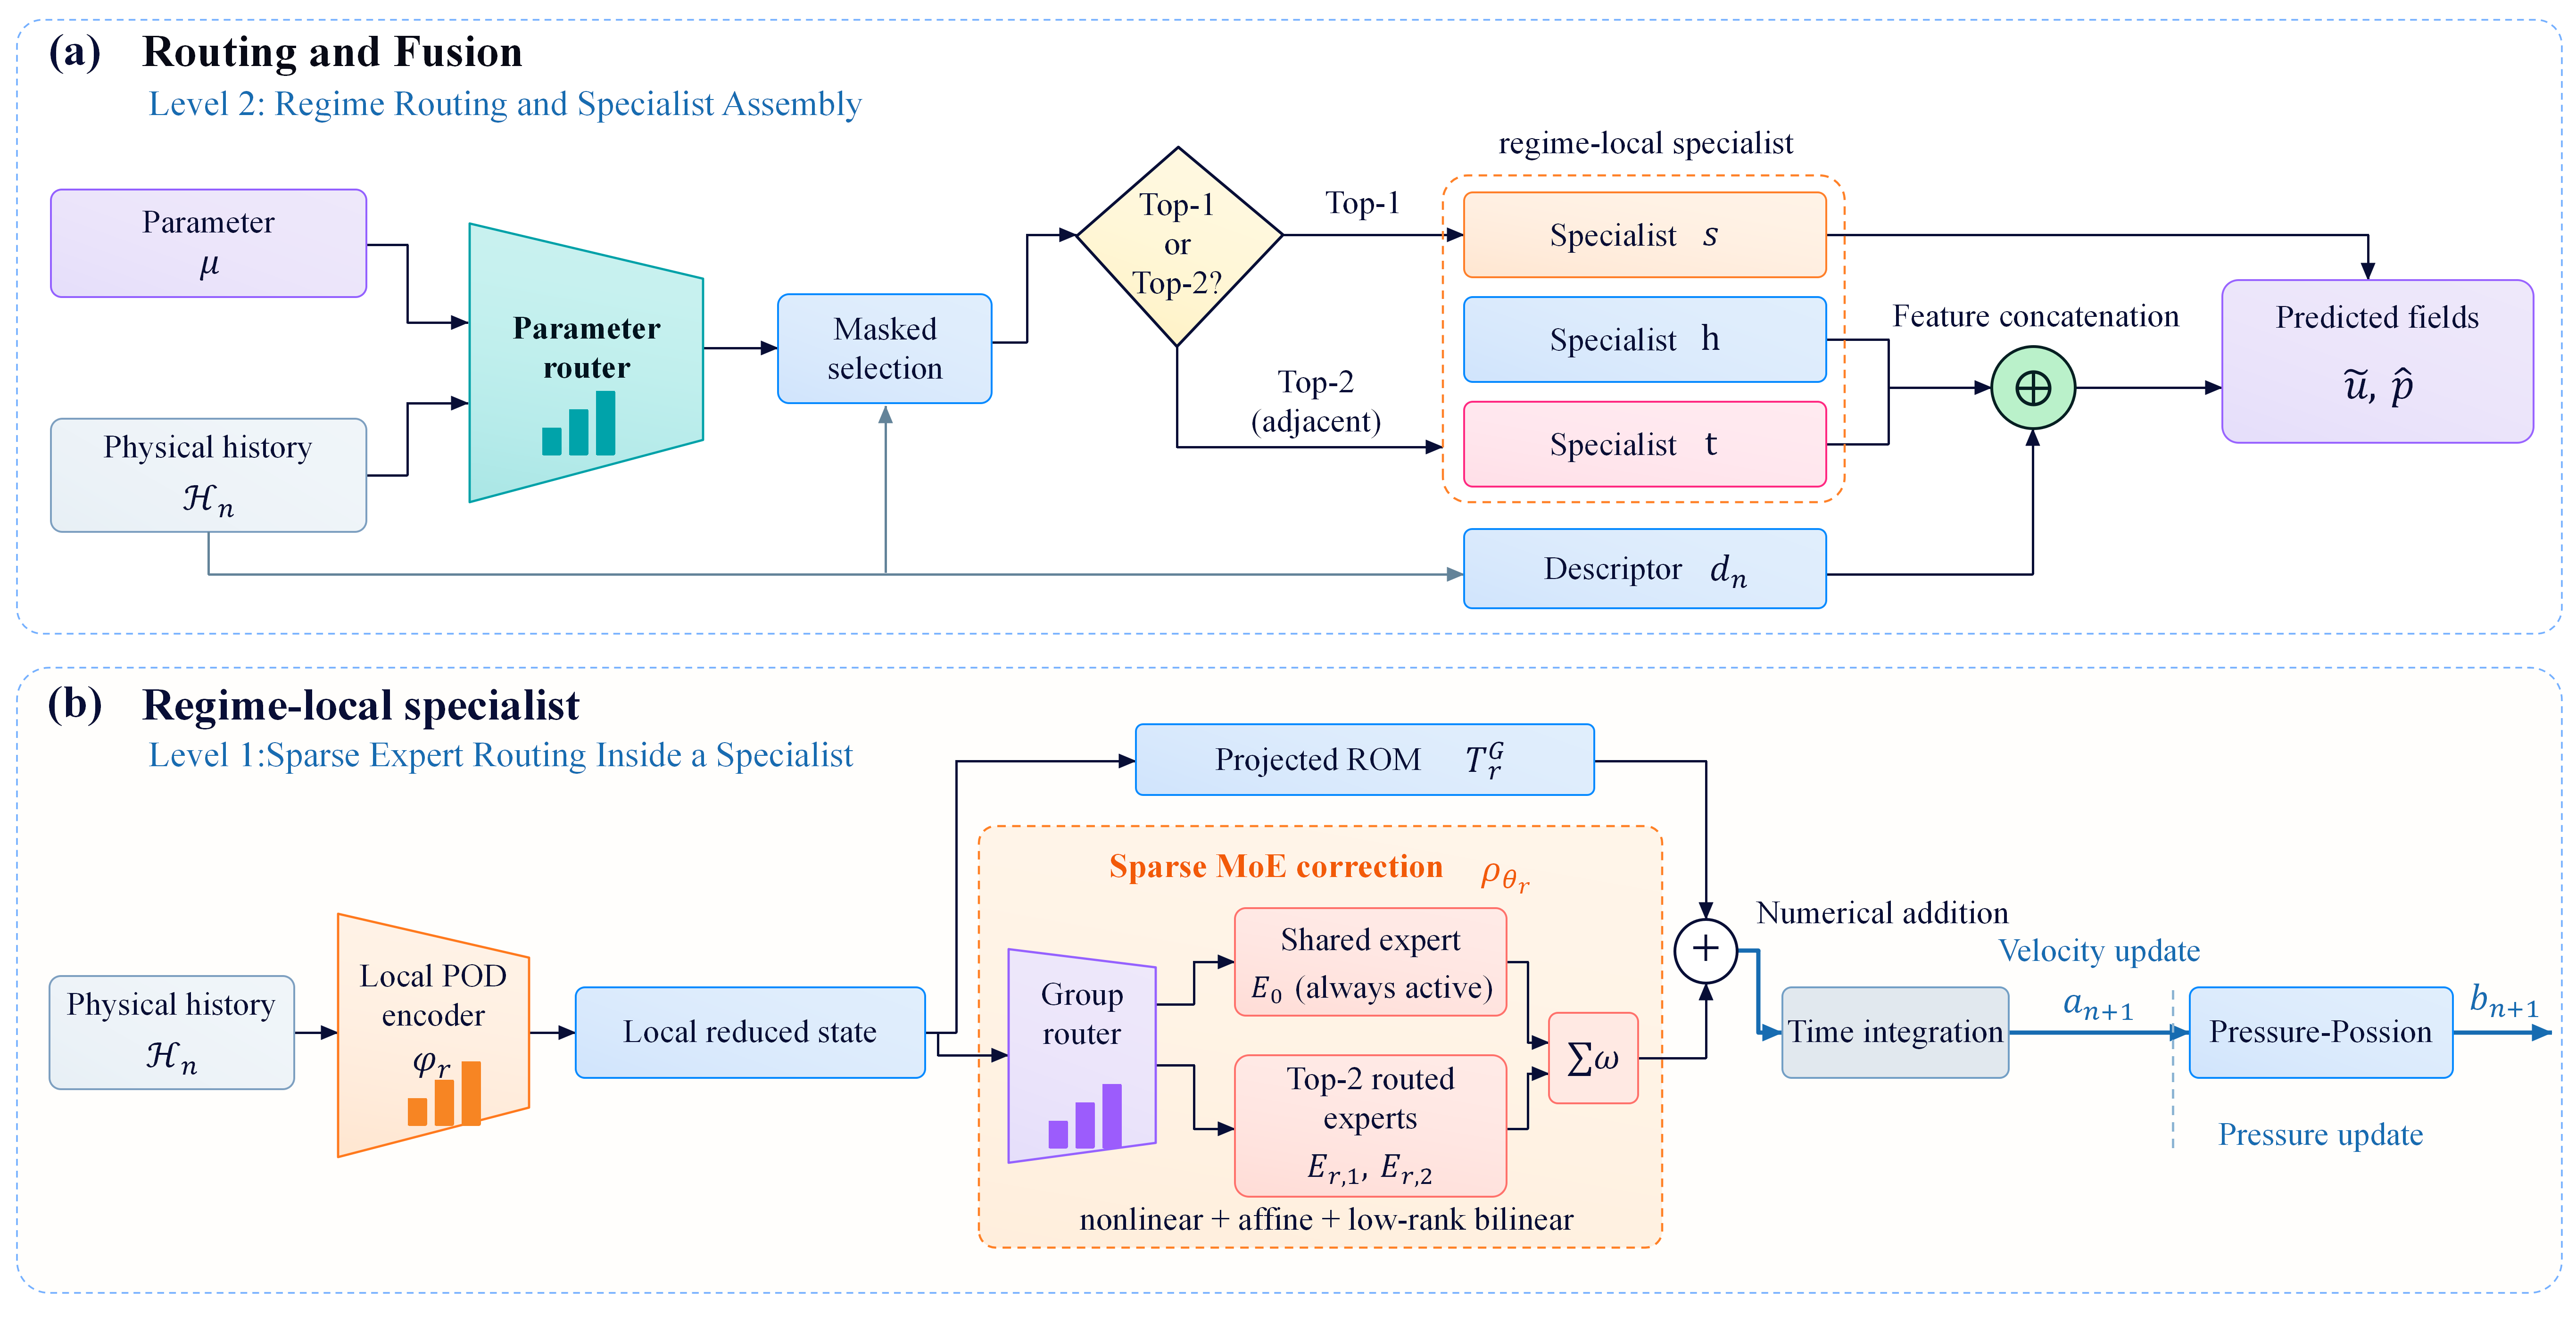
\includegraphics[width=\linewidth]{figures/flowchat.png}
\caption{
Overview of RAL-MoE-ROM.
(a) A parameter-only outer router provides trajectory-level preferences over regime-local specialists, while an applicability mask restricts inference to a single specialist or an adjacent pair. When an adjacent pair is used, a history-conditioned
gate combines only their reconstructed physical fields.
(b) Each regime-local specialist augments a projected ROMs  with a structured sparse MoE correction.
}
    \label{fig:ral_overview}
\end{figure}
\par



\section{Related Work}
\paragraph{Projection, learned dynamics, and autonomous rollout.}
POD--Galerkin methods project the governing equations onto a reduced basis and retain an explicit reduced dynamical system \citep{sirovich1987,berkooz1993,benner2015}. Their long-horizon accuracy can deteriorate when truncated interactions are not adequately represented, motivating closure and stabilization strategies
\citep{amsallem2012}. Non-intrusive and data-driven ROMs instead infer reduced evolution laws directly from simulation data, ranging from projection-based operator inference to neural and latent-state dynamics
\citep{peherstorfer2016,hesthaven2018,champion2019,lee2020, pan2024domain,park2024}. Operator-inference methods provide a particularly direct connection between data-driven reduced dynamics and classical projection-based ROMs \citep{peherstorfer2016}. Neural-operator approaches learn mappings between function spaces rather than explicit low-dimensional state evolution\citep{lu2021,kovachki2023}. Hybrid ROMs retain projected or physics-based structure while learning missing or unresolved reduced dynamics \citep{duraisamy2019,fresca2022,dar2023}. RAL-MoE-ROM follows this hybrid principle, but places a structured sparse-MoE correction inside each regime-local ROM and trains the resulting specialist under multi-step  autonomous rollout.



\paragraph{Localized representations and local reduced dynamics.}
Localization has been explored through parameter-dependent reduced bases, localized operators and nonlinear manifolds \citep{amsallem2008,peherstorfer2014,kaiser2014,li2021cluster,diaz2024,bhat2025}. These approaches all reduce the burden on a single global representation, differing in whether localization is performed along parameter, state, or spatial coordinates. Recent work has further emphasized explicitly local reduced dynamics. More recently, ql-ROM partitions the solution manifold into clusters, constructs an intrusive ROM within each cluster, and connects the local models through assignment and change-of-basis operations
\citep{colanera2025}. Therefore, when complete local ROMs are constructed independently, their reduced coordinates and operators need not be directly compatible, so switching or combining them requires an explicit coordination mechanism. RAL-MoE-ROM takes a different approach: instead of coordinating local models in reduced-coordinate space, it lets local specialists evolve independently in their native coordinates and combines neighboring predictions only after reconstruction in the common physical space.





\paragraph{Mixture-of-experts and cross-chart assembly.}
Classical hierarchical mixtures learn conditional expert assignments \citep{jacobs1991,jordan1994}, while sparse MoE architectures activate only a subset of experts for each input \citep{shazeer2017,fedus2022}. MoE-based conditional specialization has also been introduced into scientific machine learning, including physics-informed constraints, 
neural-operator pretraining, and PDE forecasting
\citep{ICLR2024_9aeda582,NEURIPS2024_b83fae17,
NEURIPS2025_2d23a999,ICLR2026_754612bd}. These methods demonstrate the value of conditional specialization, but do
not address routing among complete autonomous ROMs. RAL-MoE-ROM therefore applies router  at two levels: sparse experts model unresolved dynamics within each local ROM, while an outer router acts on the complete regime-local specialists. The outer level selects a single specialist or an
applicable neighboring pair, with the latter combined through a history-conditioned gate after physical reconstruction.



\section{RAL-MoE-ROM}
\label{sec:method}

RAL-MoE-ROM separates reduced modeling into three complementary components: regime-local ROMs, autonomous local specialists, and cross-regime router and fusion. These components are organized by a two-level routing hierarchy.  The hierarchy separates internal sparse expert routing within each local specialist from outer parameter-only regime routing (E2). For a prescribed adjacent candidate pair, history-conditioned Top-2 fusion (T2-C) combines independently predicted trajectories after reconstruction in physical space.
\subsection{Regime-local ROMs}
\label{sec:local_roms}

We consider parameterized incompressible flows governed by the
Navier--Stokes equations,
\begin{equation}
  \partial_t\bm u+(\bm u\cdot\nabla)\bm u
  =-\nabla p+\nu(\mu)\Delta\bm u+\bm f(\mu),
  \qquad \nabla\cdot\bm u=0,
  \label{eq:main_ns}
\end{equation}
with the initial and boundary conditions of each benchmark. Here $\bm u$ and $p$ denote velocity and pressure, $\mu$ is the physical parameter, $\nu$ is the viscosity, and $\bm f$ denotes a prescribed forcing term. In our nondimensional benchmarks, $\mu=Re$ and $\nu(\mu)=Re^{-1}$.

Finite-volume spatial discretization gives the semi-discrete momentum equation and incompressibility constraint,
\begin{equation}
  \dot{\bm u}
  =\bm f_h(\mu)+\mathcal L_h(\mu)\bm u
  -\mathcal N_h(\bm u,\bm u;\mu)-\nabla_h(\mu)p,
  \qquad \operatorname{div}_h(\mu)\bm u=0.
  \label{eq:main_semidiscrete}
\end{equation}
Here time remains continuous, while $\bm u\in\mathbb R^{N_u}$ and $p\in\mathbb R^{N_p}$ denote the discrete field vectors, using the same symbols as their continuous counterparts. The subscript $h$ denote spatial discretization: $\mathcal L_h$ and $\mathcal N_h$ represent th viscous and convective terms, $\nabla_h$ and $\operatorname{div}_h$ the gradient and divergence, and $\bm f_h$ the discrete forcing.

As $\mu$ varies, the flow can exhibit different dynamical regimes. Let $r\in\{S,H,P\}$ index steady, Hopf-onset, and periodic regimes, with corresponding overlapping parameter regions $\mathcal M_r$. For each region, we construct separate velocity and pressure bases by area-weighted proper orthogonal decomposition (POD) of  high-fidelity snapshots. The velocity basis
$\Phi_u^{(r)}$ satisfies ${\Phi_u^{(r)}}^\top M_u\Phi_u^{(r)}=I$,
where $M_u$ is the quadrature matrix. It defines the local encoding
and reconstruction
\begin{equation}
  \bm a^{(r)}={\Phi_u^{(r)}}^{\top}M_u(\bm u-\bar{\bm u}^{(r)}),\qquad
  \widehat{\bm u}^{(r)}=\bar{\bm u}^{(r)}+\Phi_u^{(r)}\bm a^{(r)},
  \label{eq:main_chart}
\end{equation}
where \(\bar{\bm u}^{(r)}\) is the local training mean and \(\bm a^{(r)} \in \mathbb{R}^{d_u^{(r)}}\) denotes the local reduced velocity coordinates for regime \(r\), with \(d_u^{(r)}\) the number of retained velocity POD modes. Pressure is first mapped to a common weighted zero-mean gauge and then encoded analogously using $\Phi_p^{(r)}$, yielding coefficients $\bm b^{(r)}$. Appendix~\ref{app:problem_pod} specifies the pressure gauge, quadrature, and weighted POD construction for this semi-discrete system.

Substituting the local velocity and pressure reconstructions into Eq.~(\plaineqref{eq:main_semidiscrete}) and projecting its momentum equation onto $\Phi_u^{(r)}$ in the $M_u$ inner product gives the Galerkin equation:
\begin{equation}
  \mathcal F_r^{G}(\bm a^{(r)},\bm b^{(r)};\mu)
  =\bm c_r(\mu)+\bm A_r(\mu)\bm a^{(r)}
  +\bm H_r(\mu):\bigl(\bm a^{(r)}\otimes\bm a^{(r)}\bigr)
  +\bm C_r^p(\mu)\bm b^{(r)},
  \label{eq:main_galerkin_backbone}
\end{equation}
where the terms collect the constant, linear, quadratic, and pressure
contributions.  Appendix~\ref{app:rom} defines these projected operators and the reduced Pressure--Poisson equation.


\subsection{Regime-local hybrid specialists}
\label{sec:hybrid_specialists}

A hybrid specialist augments the chart-local projected Galerkin equation with a learned velocity correction,
\begin{equation}
  \dot{\bm a}^{(r)}
  =\mathcal F_r^G(\bm a^{(r)},\bm b^{(r)};\mu)
   +\bm\rho^u_{\theta_r},
  \label{eq:main_specialist}
\end{equation}
and reconstructs pressure algebraically after the velocity update. 

\paragraph{Local features and two computation paths.}
Let $\bm g_n^{(r)}=
\mathcal F_r^G(\bm a_n^{(r)},\bm b_n^{(r)};\mu)$.
The chart-specific feature map constructs a standardized vector
\begin{equation}
  \bm\xi_n^{(r)}
  =\operatorname{Feat}_r\!\left(
    (\bm a_{n-\ell}^{(r)},\bm b_{n-\ell}^{(r)},
     \bm g_{n-\ell}^{(r)})_{\ell=0}^{2},\mu\right),
  \qquad
  \bm z_n^{(r)}=\operatorname{Enc}_r(\bm\xi_n^{(r)}).
  \label{eq:main_specialist_features}
\end{equation}
Features include current states, projected Galerkin equation, 
and parameter features. Standardization uses only the local
training set. 

The encoded features feed two paths: expert responses use
$[\bm z;\bm s^c]$, whereas routing uses
$\bm\chi=[\bm z;\bm\xi]$.  $c\in\{u,p\}$ denotes the velocity or pressure output channel, and
\begin{equation}
  \bm s^u=\widetilde{\bm a}^{(r)},
  \qquad
  \bm s^p=[\widetilde{\bm a}^{(r)};
            \widetilde{\bm b}^{(r)}]
  \label{eq:main_expert_state_inputs}
\end{equation}
are the current-state slices of the standardized feature vector. Time and chart indices are suppressed below for readability.

\paragraph{Expert-response path.}
For expert $e$ in group $m$, a nonlinear residual feed-forward
network $N_{e,m}^c$ first projects $[\bm z;\bm s^c]$ to its hidden representation, applies expanded residual blocks with GELU activations, and maps the result to $d_c$ outputs, with
$d_c=d_u^{(r)}$ or $d_p^{(r)}$.
This response is augmented by explicit linear and low-rank quadratic functions of the current state:
\begin{equation}
  [E_{e,m}^c(\bm z,\bm s^c)]_j
  =[N_{e,m}^c([\bm z;\bm s^c])]_j
   +[L_{e,m}^c\bm s^c]_j
   +\kappa\sum_{\ell=1}^{q_b}
    \bigl({\bm v_{e,m,j\ell}^{c,(1)}}^\top\bm s^c\bigr)
    \bigl({\bm v_{e,m,j\ell}^{c,(2)}}^\top\bm s^c\bigr).
  \label{eq:main_structured_expert}
\end{equation}
The linear map has no bias, and the two quadratic factors are
independent for each output component $j$. The verified configurations use $q_b=4$ and $\kappa=0.05$. Shared and routed experts have the same architecture but separate parameters. Thus the nonlinear branch uses history-conditioned features, while the explicit polynomial
branches act directly on local state coordinates.

\paragraph{Routing-and-weighting path.}
The group router receives $\bm\chi=[\bm z;\bm\xi]$ and computes
\begin{equation}
  \bm\ell^{\mathrm{grp}}=R_r^{\mathrm{grp}}(\bm\chi),
  \qquad
  \bm p^{\mathrm{grp}}
   =\operatorname{softmax}(\bm\ell^{\mathrm{grp}}/T_g),
  \qquad
  m^\star=\operatorname*{arg\,max}_m p_m^{\mathrm{grp}},
  \label{eq:main_group_selection}
\end{equation}
where $T_g>0$ is the group temperature. The router is a
layer-normalized MLP with a SiLU hidden activation and dropout. Selection is hard Top-1 for each sample. During training, a straight-through gate
$\widetilde{\bm q}=\operatorname{onehot}(m^\star)
-\operatorname{stopgrad}(\bm p^{\mathrm{grp}})
+\bm p^{\mathrm{grp}}$
retains hard selection in the forward pass while providing a
softmax gradient path.  Within the selected group, independent velocity and pressure routers with the same MLP form score six routed experts:
\begin{equation}
  \bm\ell^c=R_{r,m^\star}^c(\bm\chi),
  \qquad
  \bm p^c=\operatorname{softmax}(\bm\ell^c/T_c),
  \qquad
  \mathcal T_2^c=\operatorname{Top2}(\bm p^c).
  \label{eq:main_channel_selection}
\end{equation}
Here $\operatorname{Top2}$ returns the indices of the two largest scores and $T_c>0$ is the channel temperature. The shared expert $e=0$ is excluded from this competition and remains active in the selected group. Given configured shared and routed scales
$\lambda_0,\lambda_{\rm rt}>0$, the weights are
\begin{equation}
  \omega_0^c=\frac{\lambda_0}{\lambda_0+\lambda_{\rm rt}},
  \qquad
  \omega_e^c=
  \frac{\lambda_{\rm rt}}{\lambda_0+\lambda_{\rm rt}}
  \frac{p_e^c}{\sum_{j\in\mathcal T_2^c}p_j^c},
  \quad e\in\mathcal T_2^c.
  \label{eq:main_routing_weights}
\end{equation}
The implementation includes numerical safeguards in the denominators; the expression above gives the normalized mathematical rule. The two paths meet in the sparse mixture
\begin{equation}
  \mathcal M_{\theta_r}^c
  =\omega_0^c E_{0,m^\star}^c(\bm z,\bm s^c)
   +\sum_{e\in\mathcal T_2^c}
     \omega_e^c E_{e,m^\star}^c(\bm z,\bm s^c).
  \label{eq:main_inner_moe}
\end{equation}
Expert outputs are combined in standardized target coordinates and then converted using the chart-specific output scalers to the
velocity and pressure corrections $\bm\rho^u_{\theta_r}$ and
$\bm\rho^p_{\theta_r}$ in the additive instances.



\paragraph{Algebraic pressure reconstruction.}
In adaptive-gate instances, pressure is
reconstructed after the velocity update as
\begin{equation}
  \bm b_{n+1}^{(r)}
  =\bm\gamma_n^{(r)}\odot
     \mathcal Q_r^{PP}(\bm a_{n+1}^{(r)};\mu)
   +\bm\rho_n^{p,(r)},
  \qquad
  \bm\gamma_n^{(r)}
  =\operatorname{sigmoid}(\bm\eta_r^p(\bm z_n^{(r)})).
  \label{eq:main_pressure_closure}
\end{equation}
The independent confidence head $\bm\eta_r^p$ maps the shared
embedding through a 64-unit GELU hidden layer to $d_p^{(r)}$ outputs. It scales only the PPE candidate defined in Appendix~\ref{app:rom}; the learned correction is additive, not multiplied by $1-\bm\gamma_n^{(r)}$. Both terms are combined in the same unstandardized local pressure coordinates. The correction $\bm\rho_n^{p,(r)}$ uses the current encoded context; where configured, its expert state input is overridden using the updated velocity and
PPE pressure, without re-encoding the routing context.
Pressure is therefore reconstructed rather than independently
time-integrated; its output enters the subsequent local history.


\subsection{Closed-loop rollout training}
\label{sec:rollout_training}

Each specialist is initialized by encoding a physical history into its own local coordinates. It then advances autonomously, using its predicted velocity and reconstructed pressure to update the history. No reference state inside the prediction window is injected after initialization.

\paragraph{Frozen-context advancement.}
During one reduced velocity step, the pressure $\bm b_n^{(r)}$,
preceding-state history, and parameter define a fixed context
$\mathcal C_n^{(r)}$. For a trial velocity state $\bm a$, the hybrid
right-hand side and numerical update are
\begin{align}
  F_r(\bm a;\mathcal C_n^{(r)})
  &=\mathcal F_r^G(\bm a,\bm b_n^{(r)};\mu)
    +\bm\rho^u_{\theta_r}\!\left(
      \bm\xi^{(r)}(\bm a;\mathcal C_n^{(r)})\right),
    \label{eq:main_frozen_context_rhs}
    \\
  \bm a_{n+1}^{(r)}
  &=\operatorname{Step}_r\!\left(
     \bm a_n^{(r)};
     F_r(\cdot;\mathcal C_n^{(r)}),\Delta t_r\right).
    \label{eq:main_specialist_step}
\end{align}
Here $\Delta t_r$ is the reduced time step and
$\operatorname{Step}_r$ denotes the chart-specific advancement rule. For continuous-time instances, Runge--Kutta stages evaluate the velocity-dependent right-hand side with the same frozen context; each trial velocity triggers recomputation of the Galerkin right-hand side, current features, embedding, internal group selection, channel
Top-2 weights, and expert responses. Intermediate pressure outputs that may be computed by the full network forward pass are not used to advance pressure at the Runge--Kutta stages. The updated velocity is then supplied to Eq.~\eqref{eq:main_pressure_closure}, and the local history is shifted before the next step.  Benchmark-specific stepping rules are given in Appendix~\ref{app:implementation}.

\paragraph{Rollout prediction objective.}
Training unrolls the complete specialist update for $K$ steps with the following normalized coefficient prediction loss
\begin{equation}
  \mathcal L_r=\frac{1}{K}\sum_{k=1}^{K}\left[
  \frac{\left\|(\widehat{\bm a}_{n+k}^{(r)}-\bm a_{n+k}^{(r)})
  \oslash\bm\sigma_a^{(r)}\right\|_2^2}{d_u^{(r)}}
  +\frac{\left\|(\widehat{\bm b}_{n+k}^{(r)}-\bm b_{n+k}^{(r)})
  \oslash\bm\sigma_b^{(r)}\right\|_2^2}{d_p^{(r)}}\right].
  \label{eq:main_rollout_loss}
\end{equation}
Hats denote recursively predicted coefficients, while unhatted coefficients are reference targets. The dimensions $d_u^{(r)}$ and $d_p^{(r)}$ are chart-specific; the scaling vectors $\bm\sigma_a^{(r)}$ and $\bm\sigma_b^{(r)}$ are estimated from the corresponding training set, and $\oslash$ denotes componentwise division.  Progressively longer
rollout horizons expose the learned corrections to their own
accumulated prediction errors. The curricula and optimization
settings are reported in Appendix~\ref{app:implementation}, and held-out trajectory splits are listed in Table~\ref{tab:chart_splits}.

This expression defines the rollout prediction term, not every term in every training configuration. Learned group-routing configurations also employ auxiliary group-balance, entropy, and Reynolds-partition supervision terms; their activation and coefficients are configuration-dependent. 

\subsection{Cross-regime routing and fusion}
\label{sec:outer_routing}
Unlike the internal routing in Section~\ref{sec:hybrid_specialists}, the outer parameter-only regime router, denoted E2 in the experiments, produces a
preference over the regime-local specialists: 
\begin{equation}
  \widetilde\mu_R=(\mu-\mu_R)/\sigma_R,\qquad
  \bm\pi(\mu)=\operatorname{softmax}
  \bigl(\mathcal R_{E2}(\widetilde\mu_R)\bigr).
  \label{eq:main_e2_preference}
\end{equation}
\(R_{E2}\) is a simple three-layer MLP---a \(1\)--\(24\)--\(3\) MLP with 123 parameters. It is trained on chart-assigned parameter labels, so \(\bm\pi\) is a  parameter-conditioned preference. The deterministic parameter-only output is identical for windows with the same \(\mu\) and remains fixed during each rollout. The E2 normalization and training protocol are specified in Appendix~\ref{app:implementation}.

\paragraph{Prespecified adjacent candidates.}
The evaluation protocol supplies an ordered candidate pair $(r,s)=(S,H)$ or $(P,H)$ on prespecified common chart support
For the supplied pair, define
\begin{equation}
  \bar\pi_r=\frac{\pi_r}{\pi_r+\pi_s},\qquad
  \bar\pi_s=1-\bar\pi_r.
  \label{eq:main_pair_preference}
\end{equation}
E2 Top-1 selects $r$ when $\bar\pi_r\geq1/2$ and $s$ otherwise. The pair order means that the first-candidate weight always refers to Steady in the S--H study and Periodic in the H--P study.

\paragraph{History-conditioned output fusion.}

Both candidates encode the same physical initialization history
in their own charts and advance independently. We refer to their history-conditioned physical-space fusion as T2-C (history-conditioned Top-2 fusion).
Here, Top-2 denotes the two candidates in the prescribed adjacent
pair, rather than the internally routed correction experts. T2-C adjusts the parameter-only pair preference using a chart-independent descriptor of the initial physical history:

\begin{equation}
  \widehat{\bm q}_{\rm T2C}(t)
  =\alpha\,\widehat{\bm q}^{(r)}(t)
   +(1-\alpha)\widehat{\bm q}^{(s)}(t),\qquad
  \alpha=\operatorname{sigmoid}
  \left(\operatorname{logit}(\bar\pi_r^{\rm clip})
       +c_\psi([\widetilde\mu_G;\bm d_n])\right).
  \label{eq:main_t2c}
\end{equation}
Here $\bar\pi_r^{\rm clip}$ is $\bar\pi_r$ clipped to
$[10^{-6},1-10^{-6}]$, and $\bm q$ collects reconstructed velocity and gauge-corrected pressure on the common physical mesh. The eight descriptor channels $\bm d_n$ are computed from the initial three physical states, without future reference states. The gate input $[\widetilde\mu_G;\bm d_n]$ uses training-window normalization, distinct from the trajectory-label normalization $\widetilde\mu_R$ used by E2. The correction network is a $9$--$64$--$64$--$1$ MLP with SiLU hidden activations and a zero-initialized final layer. Its construction and physical-field training loss are given in Appendix~\ref{app:routing}.

The scalar $\alpha$ is computed for each prediction window and is shared by velocity and pressure throughout that window.
Unlike E2, it may differ between histories at the same parameter. Fusion acts only on reconstructed outputs and is never fed back into either candidate. This interface does not require identical internal architectures for the two local predictors.


\section{Experiments}
\label{sec:experiments}

We evaluate four distinct questions: local autonomous prediction,
cross-regime assembly, routing behavior and physical consistency,
and computational cost. The benchmarks have complementary roles,
not an identical matrix of experiments. Fluidic pinball provides an
archived comparison with POD--Galerkin; the circular cylinder provides
controlled local-model comparisons; and the centered square provides
the principal fusion ablations. Benchmark configurations are given in
Table~\ref{tab:chart_splits}.

\paragraph{Evaluation scope.}
We denote the joint physical-field error by $E_{\mathrm{joint}}=E_u+E_p$.
The Circular controls and Square fusion study use full-window errors
against POD-reconstructed reference fields, excluding the raw-field
projection remainder. Square terminal-step errors are supplementary
and are not mixed with full-window averages. Neural local-model seeds,
gate-only seeds, and frozen-model diagnostics are reported separately.
The experimental appendices follow the same four-part order and provide
protocols, component results, and supplementary diagnostics.



\subsection{Local prediction accuracy and finite-horizon reliability}
\label{sec:exp_local}

\paragraph{Pinball: archived prediction versus POD--Galerkin.}
Table~\ref{tab:pinball_autonomous} compares archived learned local
predictors with POD--Galerkin over $K=32$--$56$ steps. In the three
settings with a recorded baseline, the learned predictor has lower
velocity and pressure errors. The Steady baseline is unavailable.
The Periodic learned predictor is identified as Deep-FNN-H3; the
architecture of the earlier standalone Steady/Hopf rows is not fully
resolved. We therefore retain this comparison as evidence about the
archived predictors, not as an ablation attributing improvement to
sparse MoE. Appendix~\ref{app:pinball} specifies the provenance and
Periodic-core cadence. These finite-horizon results do not establish
arbitrary-time stability.


\begin{table}[H]
\centering
\caption{
Archived autonomous prediction on fluidic pinball. Errors are
physical-field percentages. ``Archived learned'' does not assert a
verified sparse-MoE architecture; the Periodic rows are Deep-FNN-H3.
Dashes denote an unavailable baseline, not divergence.
Periodic-core uses the longer evaluation in Appendix~\ref{app:pinball}.
}
\label{tab:pinball_autonomous}
\small
\setlength{\tabcolsep}{5pt}
\begin{tabular}{@{}llrrr@{}}
\toprule
Evaluation setting & Model & $E_u$ & $E_p$ & $E_{\mathrm{joint}}$ \\
\midrule
Steady ($K=56$)
& POD--Galerkin
& -- & -- & -- \\
& Archived learned
& 0.2247 & 0.7593 & 0.9840 \\
\addlinespace

Hopf ($K=56$)
& POD--Galerkin
& 0.4378 & 48.50 & 48.94 \\
& Archived learned
& 0.0995 & 1.986 & 2.085 \\
\addlinespace

Periodic ($K=32$)
& POD--Galerkin
& 1.641 & 41.56 & 43.20 \\
& Deep-FNN-H3
& 0.2897 & 0.5518 & 0.8415 \\
\addlinespace

Periodic-core ($K=56$)
& POD--Galerkin
& 2.555 & 39.36 & 41.91 \\
& Deep-FNN-H3
& 0.6222 & 1.050 & 1.672 \\
\bottomrule
\end{tabular}
\end{table}

\paragraph{Circular: controlled local architecture comparisons.}
We compare Circular Hopf and Periodic predictors on common held-out
windows at $K=24$ and $K=48$, using seeds 1248, 1600, and 2026 for
the neural configurations. This is a separate study from the Pinball
baseline comparison: it tests architecture and training sensitivity.
Dense matches the proposed model's active
neural parameter budget, while Structured retains explicit response
branches but removes input-dependent expert routing. These are
controls for the local architecture, not substitutes for a bare
POD--Galerkin ablation. We also include a validation-selected
operator inference (OpInf) fit as an external ROM comparison.
The repaired configurations change the initialization of the
low-rank quadratic factors; they are retrained models, not a
post-hoc modification of the original predictions.

Table~\ref{tab:circular_full_reorg} brings together both regimes and
horizons under the same full-window joint-error metric.
Reference fields are reconstructed from true POD coefficients, so
these errors exclude the original CFD projection remainder.
Evaluation windows, aggregation, component errors, and implementation
details are provided in Appendix~\ref{app:circular}.

\begin{table}[H]
\centering
\small
\setlength{\tabcolsep}{4pt}
\caption{Circular local controls: full-window joint error
$E_u+E_p$ (\%) against POD-reconstructed reference fields.
Neural entries are mean $\pm$ sample standard deviation over accepted
seeds among three attempts. Accepted seed sets can differ between
configurations; 2/3 rows are conditional descriptive statistics,
not complete three-seed estimates. Repaired Hopf rows use FP32.
OpInf is a single deterministic validation-selected fit.
The two horizons use the same windows, with $K=24$ restricted to
their first 24 steps.}
\label{tab:circular_full_reorg}
\begin{tabular}{@{}llccc@{}}
\toprule
Regime & Model & $K=24$ & $K=48$ & Accepted\\
\midrule
Hopf & Proposed, original
& $0.11521\pm0.08694$ & $0.11487\pm0.10033$ & 2/3\\
& Proposed, repaired
& $0.04334\pm0.02379$ & $0.05044\pm0.03439$ & 2/3\\
& Dense, active-matched
& $0.15406\pm0.16364$ & $0.15480\pm0.15525$ & 2/3\\
& Structured, original
& $0.12537\pm0.04614$ & $0.12724\pm0.04302$ & 3/3\\
& Structured, repaired
& $0.02229\pm0.00432$ & $0.02392\pm0.00778$ & 2/3\\
& OpInf & 0.03870 & 0.05340 & Deterministic\\
\midrule
Periodic & Proposed, original
& $2.8791\pm1.7269$ & $4.9443\pm3.1576$ & 3/3\\
& Proposed, repaired
& $3.0667\pm1.8373$ & $5.5322\pm3.6623$ & 3/3\\
& Dense, active-matched
& $\mathbf{1.3251\pm0.2268}$ & $\mathbf{2.3998\pm0.6599}$ & 3/3\\
& Structured, original
& $2.8666\pm1.4342$ & $5.2810\pm2.5679$ & 3/3\\
& Structured, repaired
& $2.8598\pm1.3081$ & $5.0677\pm2.3762$ & 3/3\\
& OpInf & 114.0941 & 114.9897 & Deterministic\\
\bottomrule
\end{tabular}
\end{table}

\paragraph{Architecture and external-baseline results.}
All Periodic neural configurations have three accepted seeds.
Dense yields lower mean joint errors than the proposed configurations
at both horizons, while Structured is close to the original proposed
model. Under this active-parameter budget and evaluation protocol,
the results therefore do not establish a Periodic accuracy advantage
from input-dependent sparse routing. Errors increase when extending
the window from 24 to 48 steps; neither low finite-window error nor
successful completion proves arbitrary-time stability.
The validation-selected OpInf fit is competitive on Hopf but much
less accurate on Periodic. Its Periodic ridge parameter reaches the
search-grid upper boundary; its pressure parameterization and derivative
estimation also differ from the neural models
(Appendix~\ref{app:circular}). This task-specific comparison does not
establish superiority over the OpInf method family.

\paragraph{Initialization and training reliability.}
The original Circular quadratic branches remain inactive because
both multiplicative factors were initialized at zero.
Retaining one random factor while zeroing the other permits learning,
but the repaired Proposed model does not improve the Periodic mean
error. Retraining also changes optimization and checkpoint selection,
so this comparison does not isolate the quadratic term alone.
For Hopf, repaired FP32 configurations have only two accepted seeds
per architecture, and their accepted sets differ from the original
ones. Their lower conditional errors consequently do not establish
improved expected performance or complete three-seed robustness.
Appendix~\ref{app:circular} reports the initialization mechanism and
Table~\ref{tab:hopf_completion} distinguishes training failure from
validation rejection.

\subsection{Cross-regime routing and physical-space fusion}
\label{sec:exp_fusion}

\paragraph{Square: selection and fusion controls.}
We hold the Square local predictors and E2 router fixed and compare
assembly rules on the prescribed S--H and H--P support at $K=24$.
Each interface contains 16 held-out windows.
E2 Top-1 selects within the supplied pair; T2-C learns a correction
to its pair preference using initial-history descriptors.
Neither the candidate set nor an automatic applicability mask is
learned in this experiment.

Table~\ref{tab:routing_fusion} uses a common full-window metric.
Train-fixed $\alpha$ and train-fixed logit offset are fitted only
on training windows, and the fixed candidate is selected on
validation error. These controls test whether the improvement
can be explained by a constant mixture or calibration offset.

\begin{table}[H]
\centering
\small
\caption{Square full-window joint error (\%) at $K=24$ against the
cached POD reference. Entries use the frozen-checkpoint reevaluation,
not a three-seed average. Scalar controls use training data;
the fixed candidate uses validation data.}
\label{tab:routing_fusion}
\begin{tabular}{@{}lrr@{}}
\toprule
Assembly rule & S--H & H--P\\
\midrule
E2 Top-1 & 1.5786 & 1.6424\\
E2-probability blend & 1.8145 & 1.4489\\
Equal blend & 2.3849 & 1.3930\\
Train-fixed $\alpha$ & 2.0591 & 0.9767\\
Train-fixed logit offset & 2.0149 & 0.9821\\
Validation-fixed candidate & 1.5786 & 1.0068\\
T2-C & \textbf{1.0954} & \textbf{0.8123}\\
\bottomrule
\end{tabular}
\end{table}

\paragraph{Square: history conditioning and gate variability.}
T2-C improves on all listed controls for these fixed candidate
sets. A separate architecture-matched $\mu$-only control zeros the
standardized history channels while retaining the gate architecture.
Across three paired gate seeds, full-window joint errors are
$1.095351\pm0.000015\%$ versus $1.814699\pm0.000242\%$
in S--H and $0.812343\pm0.000177\%$ versus
$0.976939\pm0.000179\%$ in H--P.
The reductions are $39.64\%$ and $16.85\%$.
These quantify gate-training variability, not uncertainty from
retraining the complete hierarchy.

\begin{figure}[H]
\centering
% Source: audited three-gate-seed full-window means; no field pixels generated.
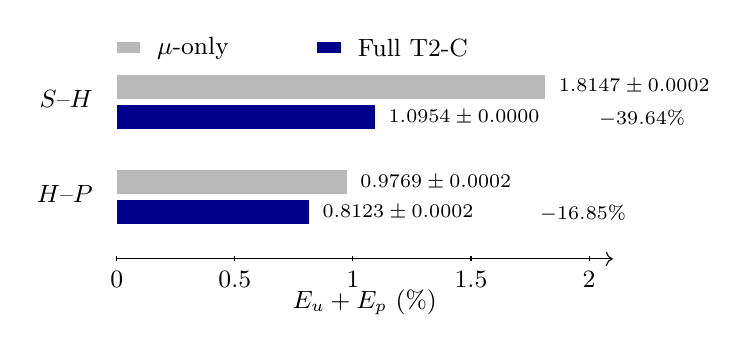
\begin{tikzpicture}[x=3cm,y=0.55cm,font=\small]
\draw[->] (0,0)--(2.1,0);
\node at (1.05,-1.0) {$E_u+E_p$ (\%)};
\foreach \t in {0,0.5,1,1.5,2} {
 \draw (\t,0.06)--(\t,-0.06) node[below] {\t};
}
\node[anchor=east] at (-0.06,3.7) {$S$--$H$};
\node[anchor=east] at (-0.06,1.5) {$H$--$P$};
\fill[gray!55] (0,3.7) rectangle (1.814699,4.25);
\fill[blue!55!black] (0,3.0) rectangle (1.095351,3.55);
\fill[gray!55] (0,1.5) rectangle (0.976939,2.05);
\fill[blue!55!black] (0,0.8) rectangle (0.812343,1.35);
% Display precision only; bar geometry retains the original means.
% The displayed 0.0000 is rounded from a nonzero standard deviation.
\node[anchor=west,font=\scriptsize] at (1.83,3.975) {$1.8147\pm0.0002$};
\node[anchor=west,font=\scriptsize] at (1.11,3.275) {$1.0954\pm0.0000$};
\node[anchor=west,font=\scriptsize] at (0.99,1.775) {$0.9769\pm0.0002$};
\node[anchor=west,font=\scriptsize] at (0.83,1.075) {$0.8123\pm0.0002$};
\fill[gray!55] (0,4.75) rectangle (0.1,5.0);
\node[anchor=west] at (0.13,4.87) {$\mu$-only};
\fill[blue!55!black] (0.85,4.75) rectangle (0.95,5.0);
\node[anchor=west] at (0.98,4.87) {Full T2-C};
\node[anchor=west,font=\scriptsize] at (2.0,3.25) {$-39.64\%$};
\node[anchor=west,font=\scriptsize] at (1.75,1.05) {$-16.85\%$};
\end{tikzpicture}

\caption{Full-window Square comparison over three paired gate seeds.
All local candidates and E2 are fixed; bars show mean and sample
standard deviation.}
\label{fig:square_overlap}
\end{figure}

The evidence supports history-conditioned fusion for these windows,
but does not prove that history dependence is necessary for every
flow or gate. The weight is fixed within each prediction window;
history can change it between windows.
Appendices~\ref{app:square}--\ref{app:square_terminal} retain component errors, terminal-step
results, scalar objectives, and complete field visualizations.
A posteriori convex oracles are diagnostics, not deployable methods.

\paragraph{Pinball: supplementary transfer of the assembly rule.}
Appendix~\ref{app:pinball_overlap_results} reports S--H and H--P
overlap results at $K=24,56$. T2-C improves on the better individual
candidate in all four archived settings. The local candidates are
Deep-FNN-H3, so these results test physical-space assembly rather than
the sparse-MoE architecture. They do not replicate the full Square
scalar-control and gate-seed study.

\paragraph{Physical-field diagnostics of fusion.}
On Square, T2-C reduces the offline pressure residual relative to
both candidates, but does not consistently improve momentum
residuals or kinetic-energy accuracy.
Appendix~\ref{app:fusion_measured} reports the comparisons and
fusion-induced defects; these reconstructed-field diagnostics
do not establish native CFD conservation.

% Replace the entire old Section 4.3, up to but excluding the cost subsection.
% Physical-field diagnostics now belong to Section 4.2 and its appendix.
\subsection{Internal expert routing and utilization}
\label{sec:exp_diagnostics}

We examine which correction experts are selected and how their weights
are allocated within the frozen original Circular H/P specialists,
distinct from E2 selection between regime-local specialists.
Periodic uses 18/18 velocity experts and 14/18 pressure experts across
the evaluated windows, with 33 and 16 distinct group--pair combinations,
respectively. Hopf has one group by construction and selects a fixed
Top-2 pair in each channel on these windows, while retaining nonuniform
weights and parameter-dependent pressure allocation.
Thus the observed behavior ranges from broad expert utilization to
fixed-support mixing; utilization alone does not establish an accuracy
advantage or physical specialization.
Appendix~\ref{app:internal_routing} provides the sampling protocol,
selection and weight statistics, and parameter- and rollout-position
profiles. These post-hoc diagnostics use different windows from the
controlled local comparisons and do not assess the repaired three-seed
configurations.

% Replace the existing computational-cost subsection.
\subsection{Computational cost and timing boundaries}
\label{sec:exp_cost}

We distinguish parameter utilization, measured local inference latency,
and a historical CFD time reference. Circular H/P activate $44.53\%$
and $17.09\%$ of their trainable parameters per prediction-path decision.
However, for Circular Periodic at batch size one and $K=48$, median
local prediction times are $2.1848$ s (proposed), $0.6579$ s (Dense),
and $0.8652$ s (Structured): sparse activation does not yield a runtime
advantage in the current implementation.
A separate measurement including physical-history encoding takes
$2.18747$ s, compared with $1996$ s for a historical FOM run over the
same physical interval. The resulting ratio of approximately $912.5$
is a historical FOM/warm-specialist comparison, not a complete-system
speedup, because hardware and I/O boundaries differ and outer routing
and fusion are excluded. Appendix~\ref{app:parameter_counts} specifies
the counting conventions, timing protocols, and comparison boundaries.

\FloatBarrier
\section{Conclusion}
We introduced RAL-MoE-ROM to combine autonomous regime-local predictors
through physical-space assembly while retaining independent reduced
coordinates. On the evaluated centered-square overlaps, physical-history
conditioning improves T2-C over the architecture-matched parameter-only
gate for all three gate-training seeds. The local control experiments
qualify the role of the inner architecture: the active-parameter-matched
Dense control is more accurate on Circular Periodic, and the original
audited quadratic branches remained inactive. Repaired Hopf training
also retains failed seeds. These results support the evaluated local
prediction and output-assembly capabilities, but do not establish sparse
routing or explicit quadratic corrections as necessary sources of
accuracy. The study assumes prescribed regime coverage and supplied
initial physical histories. Full-field CFD errors, nonlinear
constraint preservation, global cross-chart data-role verification,
and end-to-end FOM speedups remain to be established.


\subsubsection*{Reproducibility statement}
The main text reports the benchmark roles, evaluation horizons, baselines, and metrics. Appendices~\ref{app:problem_pod}--\ref{app:implementation} document the problem, projected operators, specialist architecture, routing, and implementation. Experimental appendices follow the main-text order: local prediction (Appendix~\ref{app:local_evidence}), fusion and physical-field diagnostics (Appendix~\ref{app:assembly_results}), internal expert routing (Appendix~\ref{app:routing_physics}), and cost (Appendix~\ref{app:parameter_counts}).
Appendix~\ref{app:internal_routing} reports post-hoc internal-routing statistics
from fixed validation-selected Hopf and Periodic specialists on held-out
rollout windows; these diagnostics are not used for model selection.
Appendix~\ref{app:circular} reports the new Circular control study, initialization audit, and accepted/failed seed counts; Appendix~\ref{app:parameter_counts} separates parameter counts from measured local latency.
Appendix~\ref{app:square} additionally reports an architecture-matched descriptor
ablation and three-seed variability of the centered-square T2-C gate, with the
underlying specialists and E2 router held fixed.

\subsection*{AI use statement}
% Authors must confirm this disclosure against the final submission workflow.
Generative AI tools, including ChatGPT and Codex, assisted with language polishing, LaTeX formatting, consistency checks, experiment-code development, and analysis of experimental records. The authors take full responsibility for reviewing and verifying all scientific
content, mathematical formulations, experimental configurations, numerical
results, and conclusions, and for the final manuscript and all reported results.

\bibliography{references,legacy_references}
\bibliographystyle{iclr2027_conference}

\appendix
z





\section{Full problem setup and weighted POD construction}
\label{app:problem_pod}

\subsection{Parameterized full-order model, gauge, and regime coverage}

Finite-volume spatial discretization of the Navier--Stokes equations in Eq.~(\plaineqref{eq:main_ns})  yields a semi-discrete system,as  in Eq.~(\plaineqref{eq:main_semidiscrete}),   governing the velocity
$\bm u(t;\mu)\in\mathbb R^{N_u}$ and pressure
$p(t;\mu)\in\mathbb R^{N_p}$:
\begin{equation}
    \dot{\bm u}
    =
    \bm f_h(\mu)
    +\mathcal L_h(\mu)\bm u
    -\mathcal N_h(\bm u,\bm u;\mu)
    -\nabla_h(\mu)p,
    \qquad
    \operatorname{div}_h(\mu)\bm u=0.
    \label{eq:app_fom}
\end{equation}
Here $\mathcal L_h$ and $\mathcal N_h$ denote the spatially discretized viscous and convective operators, while $\nabla_h$ and $\operatorname{div}_h$ denote the pressure gradient and velocity divergence operators. The dot denotes a continuous-time derivative; time advancement of the reduced model is specified in Section~\ref{sec:hybrid_specialists}.
Pressure is defined only up to an additive constant. With positive finite-volume weights $\bm w$, each pressure snapshot is mapped to the weighted zero-mean gauge
\begin{equation}
    \Gamma_p(q)
    =
    q-\frac{\bm w^\top q}{\bm w^\top\bm 1}\bm 1,
    \qquad
    p^\circ=\Gamma_p(p),
    \qquad
    \bm w^\top p^\circ=0.
    \label{eq:app_pressure_gauge}
\end{equation}

The parameter domain is covered by overlapping regime-local parameter regions,
\begin{equation}
    \mathcal M
    \subseteq
    \bigcup_{r\in\{S,H,P\}}\mathcal M_r,
    \qquad
    \mathcal O_{SH}
    =
    \mathcal M_S\cap\mathcal M_H,
    \qquad
    \mathcal O_{HP}
    =
    \mathcal M_H\cap\mathcal M_P,
    \label{eq:app_regime_cover}
\end{equation}
where $S$, $H$, and $P$ denote the steady, Hopf-onset, and periodic regimes, respectively. Only adjacent overlaps are used; no direct $S$--$P$ overlap is considered.


\subsection{Area-weighted local POD}

The finite-volume quadrature induces the weighted inner products
\begin{equation}
    \langle\bm v,\bm z\rangle_{M_u}
    =
    \bm v^\top M_u\bm z,
    \qquad
    \langle q,s\rangle_{M_p}
    =
    q^\top M_p s,
    \qquad
    M_p=\operatorname{diag}(\bm w),
    \qquad
    M_u=\operatorname{diag}(M_p,M_p).
    \label{eq:app_weighted_inner_products}
\end{equation}

For chart $r$, let $d_u^{(r)}$ and $d_p^{(r)}$ denote the retained velocity and pressure dimensions. Let $X_u^{(r)}$ and $X_p^{(r)}$ collect the centered velocity and gauge-corrected pressure snapshots from the training trajectories assigned to that chart. The corresponding chart-specific means are denoted by
$\bar{\bm u}^{(r)}$ and $\bar p^{(r),\circ}$.
The local POD bases solve
\begin{align}
    \Phi_u^{(r)}
    &\in
    \underset{\Psi^\top M_u\Psi=I_{d_u^{(r)}}}
    {\operatorname{arg\,min}}
    \left\|
        X_u^{(r)}
        -\Psi\Psi^\top M_uX_u^{(r)}
    \right\|_{M_u,F}^2,
    \\
    \Phi_p^{(r)}
    &\in
    \underset{\Psi^\top M_p\Psi=I_{d_p^{(r)}}}
    {\operatorname{arg\,min}}
    \left\|
        X_p^{(r)}
        -\Psi\Psi^\top M_pX_p^{(r)}
    \right\|_{M_p,F}^2,
    \label{eq:app_pod_optimization}
\end{align}
where
\begin{equation}
    \|Y\|_{M,F}^2=\operatorname{tr}(Y^\top MY).
\end{equation}

Equivalently, consider the weighted singular value decompositions
\begin{equation}
    M_u^{1/2}X_u^{(r)}
    =
    U_u^{(r)}\Sigma_u^{(r)}{V_u^{(r)}}^\top,
    \qquad
    M_p^{1/2}X_p^{(r)}
    =
    U_p^{(r)}\Sigma_p^{(r)}{V_p^{(r)}}^\top.
\end{equation}
The retained bases are
\begin{equation}
    \Phi_u^{(r)}
    =
    M_u^{-1/2}
    U_u^{(r)}(:,1{:}d_u^{(r)}),
    \qquad
    \Phi_p^{(r)}
    =
    M_p^{-1/2}
    U_p^{(r)}(:,1{:}d_p^{(r)}),
    \label{eq:app_weighted_svd_bases}
\end{equation}
and satisfy
\begin{equation}
    {\Phi_u^{(r)}}^\top M_u\Phi_u^{(r)}=I,
    \qquad
    {\Phi_p^{(r)}}^\top M_p\Phi_p^{(r)}=I.
\end{equation}
Because the pressure snapshots and their chart mean satisfy the same weighted gauge condition, the pressure basis also satisfies
\begin{equation}
    \bm w^\top\Phi_p^{(r)}=\bm 0^\top .
\end{equation}

Encoding and decoding are performed independently within each chart:
\begin{align}
    \bm a^{(r)}
    &=
    {\Phi_u^{(r)}}^\top
    M_u
    \bigl(\bm u-\bar{\bm u}^{(r)}\bigr),
    &
    \mathcal D_r^u(\bm a^{(r)})
    &=
    \bar{\bm u}^{(r)}
    +\Phi_u^{(r)}\bm a^{(r)},
    \\
    \bm b^{(r)}
    &=
    {\Phi_p^{(r)}}^\top
    M_p
    \bigl(\Gamma_p(p)-\bar p^{(r),\circ}\bigr),
    &
    \mathcal D_r^p(\bm b^{(r)})
    &=
    \bar p^{(r),\circ}
    +\Phi_p^{(r)}\bm b^{(r)}.
    \label{eq:app_encode_decode}
\end{align}

The reduced coefficients are standardized using chart-local statistics estimated from the corresponding training trajectories:
\begin{equation}
    \widetilde{\bm a}^{(r)}
    =
    \bigl(
        \bm a^{(r)}-\bm\mu_a^{(r)}
    \bigr)
    \oslash
    \bm\sigma_a^{(r)},
    \qquad
    \widetilde{\bm b}^{(r)}
    =
    \bigl(
        \bm b^{(r)}-\bm\mu_b^{(r)}
    \bigr)
    \oslash
    \bm\sigma_b^{(r)}.
    \label{eq:app_local_scalers}
\end{equation}
Additional specialist features and their normalization are specified in Section~\ref{sec:hybrid_specialists}.








\section{Projected Galerkin and pressure operators}
\label{app:rom}

\subsection{Chart-local Galerkin momentum dynamics}

For each chart $r\in\{S,H,P\}$, substituting the chart-local affine reconstructions from Appendix~\ref{app:problem_pod} into the semi-discrete momentum equation~(\plaineqref{eq:app_fom}) and testing against the local
velocity basis in the $M_u$ inner product yields
\begin{equation}
    \dot{\bm a}^{(r)}
    =
    \bm c_r(\mu)
    +
    A_r(\mu)\bm a^{(r)}
    +
    H_r(\mu):
    \bigl(
        \bm a^{(r)}\otimes\bm a^{(r)}
    \bigr)
    +
    C_r^p(\mu)\bm b^{(r)}.
    \label{eq:app_projected_momentum}
\end{equation}
Here ``$:$'' denotes the double contraction.
For velocity modes
$\bm\phi_i^{u,(r)}$,
$i=1,\ldots,d_u^{(r)}$,
and pressure modes
$\phi_\ell^{p,(r)}$,
$\ell=1,\ldots,d_p^{(r)}$,
the projected operators are
\begin{align}
    [\bm c_r(\mu)]_i
    &=
    \Bigl\langle
        \bm\phi_i^{u,(r)},
        \bm f_h(\mu)
        +
        \mathcal L_h(\mu)\bar{\bm u}^{(r)}
        -
        \mathcal N_h
        \bigl(
            \bar{\bm u}^{(r)},
            \bar{\bm u}^{(r)};
            \mu
        \bigr)
        -
        \nabla_h(\mu)\bar p^{(r),\circ}
    \Bigr\rangle_{M_u},
    \\
    [A_r(\mu)]_{ij}
    &=
    \Bigl\langle
        \bm\phi_i^{u,(r)},
        \mathcal L_h(\mu)\bm\phi_j^{u,(r)}
        -
        \mathcal N_h
        \bigl(
            \bar{\bm u}^{(r)},
            \bm\phi_j^{u,(r)};
            \mu
        \bigr)
        -
        \mathcal N_h
        \bigl(
            \bm\phi_j^{u,(r)},
            \bar{\bm u}^{(r)};
            \mu
        \bigr)
    \Bigr\rangle_{M_u},
    \\
    [H_r(\mu)]_{ijk}
    &=
    -
    \Bigl\langle
        \bm\phi_i^{u,(r)},
        \mathcal N_h
        \bigl(
            \bm\phi_j^{u,(r)},
            \bm\phi_k^{u,(r)};
            \mu
        \bigr)
    \Bigr\rangle_{M_u},
    \\
    [C_r^p(\mu)]_{i\ell}
    &=
    -
    \Bigl\langle
        \bm\phi_i^{u,(r)},
        \nabla_h(\mu)\phi_\ell^{p,(r)}
    \Bigr\rangle_{M_u}.
    \label{eq:app_projected_operators}
\end{align}

We denote the resulting chart-local projected momentum vector field by
\begin{equation}
    \mathcal F_r^G
    \bigl(
        \bm a^{(r)},
        \bm b^{(r)};
        \mu
    \bigr)
    =
    \bm c_r(\mu)
    +
    A_r(\mu)\bm a^{(r)}
    +
    H_r(\mu):
    \bigl(
        \bm a^{(r)}\otimes\bm a^{(r)}
    \bigr)
    +
    C_r^p(\mu)\bm b^{(r)}.
    \label{eq:app_galerkin_backbone}
\end{equation}
This is the projected Galerkin equation summarized in
Eq.~(\plaineqref{eq:main_galerkin_backbone}); the additive hybrid specialist augments it with the learned closure in Eq.~(\plaineqref{eq:main_specialist}).


\subsection{Reduced pressure--Poisson equation}
\label{app:reduced_ppe}

Taking the divergence of the incompressible momentum equation with spatially constant viscosity gives
\begin{equation}
    -\Delta p^\circ
    =
    \nabla\cdot\bigl[(\bm u\cdot\nabla)\bm u-\bm f\bigr],
    \qquad
    \int_\Omega p^\circ\,\mathrm d\Omega=0,
    \label{eq:app_ppe}
\end{equation}
where $p^\circ$ denotes gauge-corrected pressure. Substituting \eqref{eq:app_encode_decode} into \eqref{eq:app_ppe}, and applying local pressure-mode testing, integration by parts, and Appendix~A quadrature for the volume integrals, yields a reduced pressure system.

\begin{equation}
    K_r^p(\mu)\bm b^{PP,(r)}
    =
    \bm d_r(\mu)
    +B_r(\mu)\bm a^{(r)}
    +Q_r(\mu):
    \bigl(\bm a^{(r)}\otimes\bm a^{(r)}\bigr),
    \label{eq:app_pressure_poisson_system}
\end{equation}
where
\begin{align}
    [K_r^p]_{\ell m}
    &=
    -\bigl\langle
        \nabla_h\phi_\ell^{p,(r)},
        \nabla_h\phi_m^{p,(r)}
    \bigr\rangle_{M_u},
    \label{eq:app_ppe_K_definition}
    \\
    [\bm d_r]_\ell
    &=
    \bigl\langle
        \nabla_h\phi_\ell^{p,(r)},
        \mathcal N_h(\bar{\bm u}^{(r)},\bar{\bm u}^{(r)};\mu)
        -\bm f_h(\mu)
        +\nabla_h\bar p^{(r),\circ}
    \bigr\rangle_{M_u},
    \label{eq:app_ppe_d_definition}
    \\
    [B_r]_{\ell j}
    &=
    \bigl\langle
        \nabla_h\phi_\ell^{p,(r)},
        \mathcal N_h(\bar{\bm u}^{(r)},\phi_j^{u,(r)};\mu)
        +\mathcal N_h(\phi_j^{u,(r)},\bar{\bm u}^{(r)};\mu)
    \bigr\rangle_{M_u},
    \label{eq:app_ppe_B_definition}
    \\
    [Q_r]_{\ell jk}
    &=
    \bigl\langle
        \nabla_h\phi_\ell^{p,(r)},
        \mathcal N_h(\phi_j^{u,(r)},\phi_k^{u,(r)};\mu)
    \bigr\rangle_{M_u}.
    \label{eq:app_ppe_Q_definition}
\end{align}


The resulting algebraic pressure map is
\begin{equation}
    \mathcal Q_r^{PP}(\bm a^{(r)};\mu)
    =
    \bigl(K_r^p(\mu)\bigr)^\dagger
    \left[
        \bm d_r(\mu)
        +B_r(\mu)\bm a^{(r)}
        +Q_r(\mu):
        \bigl(\bm a^{(r)}\otimes\bm a^{(r)}\bigr)
    \right],
    \label{eq:app_pressure_poisson_map}
\end{equation}
where ${}^\dagger$ denotes the Moore--Penrose pseudoinverse and  coincides with the inverse when $K_r^p$ is nonsingular.
The pressure field is then reconstructed as
$\mathcal Q_r^{PP}(\bm a^{(r)};\mu)$.
Thus, pressure is recovered algebraically from the local velocity state rather than advanced as an independent dynamical variable.



% \section{Regime-local specialist architecture and closed-loop training}
% \label{app:specialists}

% For each regime-local chart $r$, we define a self-contained 
% specialist in its native reduced coordinates: velocity is advanced
% dynamically, whereas pressure is reconstructed algebraically.
% The projected operators from Appendix~\ref{app:rom} provide the underlying physics, while learned terms model unresolved reduced dynamics. The velocity coefficients satisfy
% \begin{equation}
%   \dot{\bm a}^{(r)}
%   =
%   \mathcal F_r^G
%   \left(
%     \bm a^{(r)},\bm b^{(r)};\mu
%   \right)
%   +
%   \bm\rho^u_{\theta_r}
%   \left(
%     \bm\xi^{(r)}
%   \right).
%   \label{eq:app_hybrid_velocity_rhs}
% \end{equation}
% After each reduced velocity time step, pressure is reconstructed through
% \begin{align}
%   \bm b_{n+1}^{PP,(r)}
%   &=
%   \mathcal Q_r^{PP}
%   \left(
%     \bm a_{n+1}^{(r)};\mu
%   \right),
%   \nonumber\\
%   \bm\gamma_n^{(r)}
%   &=
%   \operatorname{sigmoid}
%   \left(
%     \bm\eta^p_{\theta_r}
%     (\bm\xi_n^{(r)})
%   \right),
%   \nonumber\\
%   \bm b_{n+1}^{(r)}
%   &=
%   \bm\gamma_n^{(r)}
%   \odot
%   \bm b_{n+1}^{PP,(r)}
%   +
%   \bm\rho^p_{\theta_r}
%   (\bm\xi_n^{(r)}),
%   \qquad
%   \bm\gamma_n^{(r)}
%   \in(0,1)^{d_p^{(r)}}.
%   \label{eq:app_pressure_closure}
% \end{align}
% The gate modulates the projected Pressure--Poisson contribution, while
% $\bm\rho^p_{\theta_r}$ provides the learned pressure correction.


% \subsection{Features and structured sparse experts}

% Let
% \begin{equation}
%   \bm g_n^{(r)}
%   =
%   \mathcal F_r^G
%   \left(
%     \bm a_n^{(r)},\bm b_n^{(r)};\mu
%   \right)
%   \label{eq:app_galerkin_feature}
% \end{equation}
% denote the projected velocity right-hand side defined in Eq.~(\plaineqref{eq:app_galerkin_backbone}). The specialist uses the ordered three-state history
% \begin{equation}
%   \mathcal H_n^{(r)}
%   =
%   \left(
%     \bm a_{n-\ell}^{(r)},
%     \bm b_{n-\ell}^{(r)},
%     \bm g_{n-\ell}^{(r)}
%   \right)_{\ell=0}^{2},
%   \label{eq:app_specialist_history}
% \end{equation}
% and constructs
% \begin{equation}
%   \bm\xi_n^{(r)}
%   =
%   \operatorname{Feat}_r
%   \left(
%     \mathcal H_n^{(r)},\mu
%   \right),
%   \qquad
%   \bm z_n^{(r)}
%   =
%   \operatorname{Enc}_r
%   \left(
%     \bm\xi_n^{(r)}
%   \right).
%   \label{eq:app_specialist_features}
% \end{equation}
% The feature map contains standardized local states, projected
% right-hand sides and parameter features. All normalization statistics are estimated from the corresponding chart-specific training set. Internal routing first selects an expert group. When group selection is learned,
% \begin{equation}
%   m^\star
%   =
%   \underset{m\in\mathcal G_r}{\operatorname{arg\,max}}
%   \;
%   \pi_{r,m}^{\mathrm{grp}}
%   \left(
%     \bm z_n^{(r)},\bm\xi_n^{(r)}
%   \right),
%   \label{eq:app_group_top1}
% \end{equation}
% whereas $m^\star$ is predetermined for single-group or fixed-group
% specialists. Within the selected group, velocity and pressure use separate channel routers. For $c\in\{u,p\}$, let $\mathcal T_2^c$ denote the two routed experts with the largest channel-specific weights. Together with the shared expert $e=0$,
% \begin{equation}
%   \mathcal M_{\theta_r}^c
%   =
%   \omega_0^c
%   E_{0,m^\star}^c
%   +
%   \sum_{e\in\mathcal T_2^c}
%   \omega_e^c
%   E_{e,m^\star}^c,
%   \qquad
%   \omega_e^c\ge0,
%   \qquad
%   \omega_0^c+\sum_{e\in\mathcal T_2^c}\omega_e^c=1.
%   \label{eq:app_channel_sparse_moe}
% \end{equation}
% The two channel mixtures define the velocity and pressure corrections
% $\bm\rho_{\theta_r}^u$ and $\bm\rho_{\theta_r}^p$, respectively. The explicit linear and quadratic branches operate on the channel-specific reduced-state inputs
% \begin{equation}
%   \bm s^{u,(r)}
%   =
%   \widetilde{\bm a}^{(r)},
%   \qquad
%   \bm s^{p,(r)}
%   =
%   \operatorname{col}
%   \left(
%     \widetilde{\bm a}^{(r)},
%     \widetilde{\bm b}^{(r)}
%   \right).
%   \label{eq:app_expert_state_slices}
% \end{equation}
% For output component $j$, each expert is
% \begin{align}
%   \left[E_{e,m}^c\right]_j
%   &=
%   \left[
%     N_{e,m}^c
%     \left(
%       \bm z,\bm s^c
%     \right)
%   \right]_j
%   +
%   \left[
%     W_{e,m}^{c,\mathrm{lin}}
%     \bm s^c
%   \right]_j
%   \nonumber\\
%   &\quad+
%   \kappa
%   \sum_{\ell=1}^{q_b}
%   \left(
%     {\bm u_{e,m,j\ell}^c}^{\top}
%     \bm s^c
%   \right)
%   \left(
%     {\bm v_{e,m,j\ell}^c}^{\top}
%     \bm s^c
%   \right),
%   \qquad
%   q_b=4,
%   \qquad
%   \kappa=0.05.
%   \label{eq:app_structured_expert}
% \end{align}
% Thus each expert combines a nonlinear feature-conditioned response with
% explicit linear and low-rank quadratic responses of the local reduced state.


% \subsection{Frozen-context advancement and closed-loop training}

% During one reduced velocity time step, the current pressure, recent history, and
% physical parameter define a context $\mathcal C_n^{(r)}$ that is held fixed
% while the velocity state is advanced. We write
% \begin{equation}
%   F_r
%   \left(
%     \bm a;\mathcal C_n^{(r)}
%   \right)
%   =
%   \mathcal F_r^G
%   \left(
%     \bm a,\bm b_n^{(r)};\mu
%   \right)
%   +
%   \bm\rho^u_{\theta_r}
%   \left(
%     \bm\xi^{(r)}
%     \left(
%       \bm a;\mathcal C_n^{(r)}
%     \right)
%   \right).
%   \label{eq:app_frozen_context_rhs}
% \end{equation}
% The chart-specific numerical update is denoted by
% \begin{equation}
%   \bm a_{n+1}^{(r)}
%   =
%   \operatorname{Step}_r
%   \left(
%     \bm a_n^{(r)};
%     F_r(\cdot;\mathcal C_n^{(r)}),
%     \Delta t_r
%   \right).
%   \label{eq:app_specialist_step}
% \end{equation}
% Continuous-time specialist instances use Runge--Kutta integration with the
% same frozen context across stage evaluations; benchmark-specific stepping
% details are reported in Appendix~\ref{app:implementation}.
% The updated velocity is then supplied to
% Eq.~(\plaineqref{eq:app_pressure_closure}), after which the history is
% shifted and autonomous rollout continues.

% For a closed-loop rollout of length $K$, the specialist recursively
% consumes its own predicted states and minimizes
% \begin{equation}
%   \mathcal L_r
%   =
%   \frac{1}{K}
%   \sum_{k=1}^{K}
%   \left[
%     \frac{1}{d_u^{(r)}}
%     \left\|
%       \left(
%         \widehat{\bm a}_{n+k}^{(r)}
%         -
%         \bm a_{n+k}^{(r)}
%       \right)
%       \oslash
%       \bm\sigma_a^{(r)}
%     \right\|_2^2
%     +
%     \frac{1}{d_p^{(r)}}
%     \left\|
%       \left(
%         \widehat{\bm b}_{n+k}^{(r)}
%         -
%         \bm b_{n+k}^{(r)}
%       \right)
%       \oslash
%       \bm\sigma_b^{(r)}
%     \right\|_2^2
%   \right].
%   \label{eq:app_true_rollout_loss}
% \end{equation}
% After initialization, no reference state inside the prediction window is
% injected into the autonomous rollout. Training uses progressively longer
% chart-specific rollout horizons; the corresponding curricula and
% optimization settings are listed in Appendix~\ref{app:implementation}.

\section{Outer routing and T2-C details}
\label{app:routing}


\paragraph{Chart-independent physical-history descriptor.}
The implementation  in Section \ref{sec:outer_routing} uses eight descriptor channels and one parameter input. These features are computed from the initial three physical states at $t_{n-2}<t_{n-1}<t_n$, with pressure mapped to the common zero-mean gauge. They are independent of the specialists' POD coordinates. All quantities below use the nondimensional data conventions of the experiment, and $\epsilon=10^{-12}$ is the numerical floor.

Define $A_\Omega=\sum_i w_i$, $U_j=\|\bm u_j\|_{M_u}^2$, $P_j=\|p_j^\circ\|_{M_p}^2$, and
\begin{align}
 h_j&=\max(t_j-t_{j-1},\epsilon),&
 s_j^u&=\sqrt{\max(U_j,\epsilon)},&
 s_j^p&=\sqrt{\max(P_j,\epsilon)},\\
 v_j&=(\bm u_j-\bm u_{j-1})/h_j,&
 g_j&=\frac{\log\max(U_j,\epsilon)-\log\max(U_{j-1},\epsilon)}{h_j}.
\end{align}
The ordered raw descriptor is
\begin{equation}
\bm s_n=\operatorname{col}\left(
\begin{array}{l}
 \tfrac12\log\max(U_n/A_\Omega,\epsilon),\\
 \tfrac12\log\max(P_n/A_\Omega,\epsilon),\\
 \log(1+\|v_n\|_{M_u}/(s_n^u+\epsilon)),\\
 \log(1+\|v_{n-1}\|_{M_u}/(s_{n-1}^u+\epsilon)),\\
 \tanh(g_n),\\
 \tanh(g_n-g_{n-1}),\\
 \log(1+\|p_n^\circ-p_{n-1}^\circ\|_{M_p}/[h_n(s_n^p+\epsilon)]),\\
 \log(1+\|v_n-v_{n-1}\|_{M_u}/(s_n^u+\epsilon))
\end{array}\right).
\label{eq:app_t2c_descriptor}
\end{equation}
The last channel measures a difference of velocity rates: it is not divided again by a time interval and is not the second-derivative descriptor in an acceleration discretization. The log and hyperbolic-tangent transformations above are part of the actual feature construction. For the gate, the nine raw features $[\mu;\bm s_n]$ are standardized using the means and population standard deviations of training windows only. Any feature standard deviation below $10^{-8}$ is replaced by one. We denote the resulting vector by $[\widetilde\mu_G;\bm d_n]$; its parameter normalization is fitted for the gate and is distinct from the E2 training-row normalization $\widetilde\mu_R$. The architecture-matched $\mu$-only control sets all eight descriptor channels to zero after standardization. 


\paragraph{Physical-space T2-C fusion.}
The logit-correction network receives
$[\widetilde\mu_G;\bm d_n]\in\mathbb R^9$ and uses two hidden layers of width 64 with SiLU
activations followed by a scalar linear output (9--64--64--1; 4,865 trainable parameters).
The final layer is initialized at zero, so the initial correction vanishes
and the fusion weight reduces to the E2 pair preference.
Specifically,
\begin{equation}
  \Delta_\psi
  =
  c_\psi
  \left(
    [\widetilde\mu_G;\bm d_n]
  \right),
  \qquad
  \alpha
  =
  \operatorname{sigmoid}
  \left(
    \ell^{E2}+\Delta_\psi
  \right).
  \label{eq:app_t2c_gate}
\end{equation}

The two selected specialists encode the same physical history in their
respective local charts and then evolve independently.
The scalar $\alpha$ is fixed throughout the prediction window and is shared
by velocity and pressure.
After reconstruction on the common physical mesh, T2-C forms
\begin{equation}
  \widehat{\bm q}_{\alpha}^{\,c}(t)
  =
  \alpha\,
  \widehat{\bm q}_{1}^{\,c}(t)
  +
  (1-\alpha)\,
  \widehat{\bm q}_{2}^{\,c}(t),
  \qquad
  c\in\{u,p\},
  \label{eq:app_t2c_field_fusion}
\end{equation}
where the pressure field is gauge corrected.
The fused field is an output only and is never projected back into either
specialist.


\section{Reproducibility and implementation details}
\label{app:implementation}

\paragraph{Physical-field error metrics.}
We evaluate reconstructed velocity and gauge-corrected pressure using the relative weighted field errors
\begin{equation}
E_u(n)
=
100\frac{
\|\widehat{\bm u}_n-\bm u_n\|_{M_u}
}{
\|\bm u_n\|_{M_u}
},
\qquad
E_p(n)
=
100\frac{
\|\widehat p_n^\circ-p_n^\circ\|_{M_p}
}{
\|p_n^\circ\|_{M_p}
}.
\label{eq:field_errors}
\end{equation}
Here $\|\bm v\|_M=(\bm v^\top M\bm v)^{1/2}$ uses the finite-volume quadrature introduced in Appendix~\ref{app:problem_pod}; the velocity norm includes both components, and $p^\circ$ denotes pressure in the common zero-mean gauge. Unless stated otherwise, benchmark-specific temporal and trajectory aggregation is reported with the corresponding experiment. Whenever a joint score is reported, $E_{\mathrm{joint}}=E_u+E_p$. 


\paragraph{Trajectory-level partitioning.}
Table~\ref{tab:chart_splits} summarizes the resulting chart-wise parameter coverage, reduced dimensions, trajectory splits, and evaluation horizons. All splits are defined at the level of complete parameter trajectories rather than individual snapshots or rollout windows. Local bases, normalization statistics, and model parameters are constructed from training trajectories only.

\par
\begin{table}[H]
\centering
\caption{
Chart-wise parameter coverage, reduced dimensions, trajectory splits, and evaluation horizons. $K$ denotes the number of autonomous rollout steps used for the corresponding local evaluation.
}
\label{tab:chart_splits}
\small
\setlength{\tabcolsep}{3.5pt}
\begin{tabular}{@{}llrrrrrr@{}}
\toprule
Benchmark & Chart & $Re$ range & $(r_u,r_p)$ & Train & Val. & Test & $K$ \\
\midrule
Circular cylinder
& $S$ & 20.0--46.4 & $(32,32)$ & 14 & 2 & 4 & 56 \\
& $H$ & 45.5--59.2 & $(32,32)$ & 29 & 2 & 3 & 56 \\
& $P$ & 57.3--200 & $(32,32)$ & 53 & 6 & 4 & 48 \\
\addlinespace
Centered square
& $S$ & 50--95.4 & $(5,4)$ & 60 & 5 & 4 & 16 \\
& $H$ & 94--102 & $(11,11)$ & 23 & 6 & 5 & 48 \\
& $P$ & 98.5--150 & $(28,26)$ & 27 & 6 & 4 & 24 \\
\addlinespace
Fluidic pinball
& $S$ & 10--19 & $(4,3)$ & 37 & 8 & 7 & 56 \\
& $H$ & 16.6--25 & $(5,5)$ & 39 & 8 & 7 & 56 \\
& $P$ & 21.25--60 & $(17,16)$ & 47 & 9 & 9 & 32 \\
\bottomrule
\end{tabular}
\end{table}
\par


\paragraph{T2-C gate optimization.}
Both full T2-C and the architecture-matched $\mu$-only gate use AdamW (learning rate $3\times10^{-4}$, weight decay $10^{-4}$), 8,000 steps, and gradient-norm clipping at 1. Minibatches sample training windows with
replacement. Validation is evaluated at step 1 and every 100 steps; checkpoint selection minimizes the largest Reynolds-number-wise full-window mean joint error.
The evaluation is reported in Appendix~\ref{app:square}.





\paragraph{Benchmark discretization and sampling.}
The centered-square dataset contains 120 complete trajectories over
$Re\in[50,150]$ on a 9,400-cell finite-volume mesh. The CFD time step is $\delta t_{\rm CFD}=0.02$, and snapshots are stored every 200 CFD steps, giving $\Delta t_{\rm snap}=4$. The fluidic-pinball dataset contains 131 complete trajectories over $Re\in[10,60]$ on a 70,194-cell mesh, with $\delta t_{\rm CFD}=0.005$ and a snapshot interval of $0.25$ physical time units. The circular-cylinder dataset contains 100 Reynolds-parameterized trajectories spanning
$Re\in[20,200]$ on a common finite-volume mesh represented by 97,368 spatial points. Trajectories contain different numbers of snapshots, yielding 14,167 snapshots in total. The unsteady simulations employ adaptive CFD time stepping subject to $Co_{\max}=0.8$ and $\delta t_{\max}=0.2$, while the snapshot interval is adjusted according to the estimated vortex-shedding period, with eight snapshots retained per shedding cycle. The chart-wise parameter ranges, reduced dimensions, splits, and evaluation horizons are summarized in Table~\ref{tab:chart_splits}.


\paragraph{Specialist optimization.}
Table~\ref{tab:specialist_training} summarizes the reported training configurations, which use AdamW with chart-specific learning rates, weight decay, and rollout curricula. 

\par
\begin{table}[H]
\centering
\caption{
Reported specialist training configurations. ``Selected'' denotes the validation-selected checkpoint. The curriculum and budget describe the configured schedule, which may extend beyond the selected checkpoint.
}
\label{tab:specialist_training}
\small
\setlength{\tabcolsep}{3.5pt}
\begin{tabular}{@{}lccccc@{}}
\toprule
Specialist & Initial lr & Weight decay & Rollout curriculum & Budget & Selected \\
\midrule
Circular $S$
& $1.55{\times}10^{-5}$ & $1.0{\times}10^{-4}$
& 4,8,16 & 3600 steps & 1200 steps \\
Circular $H$
& $1.0{\times}10^{-3}$ & $1.0{\times}10^{-4}$
& 1,2,4,8 & 8000 steps & 7200 steps \\
Circular $P$
& $5.5{\times}10^{-4}$ & $1.5{\times}10^{-4}$
& 4,8,12,16 & 240 epochs & 85 epochs \\
\addlinespace
Square $S$
& $1.55{\times}10^{-5}$ & $1.0{\times}10^{-4}$
& 1,4,8,16 & 4000 steps & 3200 steps \\
Square $H$
& $1.0{\times}10^{-3}$ & $1.0{\times}10^{-4}$
& 1,2,4,8 & 8000 steps & 7200 steps \\
Square $P$
& $5.5{\times}10^{-4}$ & $1.5{\times}10^{-4}$
& 4,8,12,16 & 720 epochs & 490 epochs \\
\addlinespace
Pinball $S$
& $1.0{\times}10^{-3}$ & $1.0{\times}10^{-4}$
& 4,8,16 & 8000 steps & 400 steps \\
Pinball $H$
& $1.0{\times}10^{-3}$ & $1.0{\times}10^{-4}$
& 4,8,16,32,56 & 8000 steps & 8000 steps \\
Pinball $P$
& $1.0{\times}10^{-3}$ & $1.0{\times}10^{-4}$
& 4,8,16,24,32 & 8000 steps & 8000 steps \\
\bottomrule
\end{tabular}
\end{table}
\par



\paragraph{ Outer E2 router configuration.}
The parameter-only router is an MLP $1\to24\to3$ with a Tanh hidden activation and 123 trainable parameters. The scalar Reynolds number is standardized using training-row mean and population standard deviation; a standard deviation below $10^{-7}$ is replaced by one. Within each chart and split, each unique Reynolds number supplies one row with that chart label. A parameter occurring in more than one chart can therefore produce multiple labeled rows, rather than an assumed unique bifurcation label. The loss is class-weighted cross entropy plus $0.05\,\operatorname{mean}(\pi_S\pi_P)$, with class weight $N/(3N_c)$. Training uses AdamW (learning rate $3\times10^{-4}$, weight decay $10^{-4}$), a cosine schedule over 8,000 steps ending at $1.5\times10^{-5}$, sampling with replacement in batches of $\min(256,N)$, and gradient-norm clipping at one. Selection maximizes validation balanced accuracy plus macro-F1 minus $10^{-3}$ times the current training-batch loss, rather than validation cross entropy alone. 



\paragraph{Specialist architectures.}


For sparse MoE, $D=13+5(2d_u+d_p)$ is feature width. Features include parameter terms, current coefficients and projected Galerkin equation, 11 derived
norm/energy/ratio quantities, and two historical blocks.
The time step is an integrator input, not a network feature.
Each encoder has three linear layers of width $h$ with LayerNorm
and SiLU; the first two include dropout 0.04. Two refinement residual
blocks follow. Velocity and pressure share this encoder, but not
their router or expert parameters.


Each group contains six routed experts and one shared expert per
channel, with separate velocity/pressure Top-2 supports. Routers
receive $[\bm z;\bm\xi]$ and use LayerNorm, a width-$h$ SiLU hidden
layer, dropout 0.04, and a linear logit head. Each expert projects
$[\bm z;\bm s^c]$ to width $h$, applies $B$ expanded residual
feed-forward blocks with GELU, and maps to the channel output.
Residual scales are learned scalars initialized to 0.1.
The explicit linear branch has no bias; the two quadratic factors
each have shape $d_c\times4\times\dim(\bm s^c)$, with
$\kappa=0.05$ and no additional output projection. The branches are
added within each expert before sparse mixture weighting. Outputs
are converted from standardized target coordinates before combination
with physical-model terms.










% \paragraph{Reference fields and reporting scope.}
% The new circular-cylinder control study and centered-square cache-based
% reevaluation use POD-reconstructed reference fields. Their errors measure
% prediction error in physical space relative to these reconstructions and
% do not include the POD projection remainder relative to the original CFD
% fields. The original CFD total error and the POD projection error require
% a separate aligned-field evaluation. The nominal chart-wise splits above
% do not by themselves establish a global cross-chart data-role audit.

% \paragraph{Training and evaluation lengths.}
% The configured maximum rollout lengths in Table~\ref{tab:specialist_training}
% are $16,8,16$ for both Circular and Square $S,H,P$, and $16,56,32$ for
% Pinball $S,H,P$. These are training budgets, not the local evaluation
% horizons in Table~\ref{tab:chart_splits}. The new Circular H/P comparison
% uses $K=24,48$, while Square overlaps use $K=24$. The selected checkpoint
% may precede the end of its configured curriculum.









% \paragraph{Physical-field error metrics.}
% We evaluate reconstructed velocity and gauge-corrected pressure using the relative weighted field errors
% \begin{equation}
% E_u(n)
% =
% 100\frac{
% \|\widehat{\bm u}_n-\bm u_n\|_{M_u}
% }{
% \|\bm u_n\|_{M_u}
% },
% \qquad
% E_p(n)
% =
% 100\frac{
% \|\widehat p_n^\circ-p_n^\circ\|_{M_p}
% }{
% \|p_n^\circ\|_{M_p}
% }.
% \label{eq:field_errors}
% \end{equation}
% Here $\|\bm v\|_M=(\bm v^\top M\bm v)^{1/2}$ uses the finite-volume
% quadrature introduced in Appendix~\ref{app:problem_pod}; the velocity norm includes both components, and $p^\circ$ denotes pressure in the common zero-mean gauge. Unless stated otherwise, benchmark-specific temporal and trajectory aggregation is reported with the corresponding experiment. Whenever a joint score is reported,
% $E_{\mathrm{joint}}=E_u+E_p$. Independently rounded component values may therefore differ slightly from the displayed joint score.


% \paragraph{Trajectory-level partitioning.}
% Table~\ref{tab:chart_splits} summarizes the resulting chart-wise parameter coverage, reduced dimensions, trajectory splits, and evaluation horizons. All splits are defined at the level of complete parameter trajectories rather than individual snapshots or rollout windows. Local bases, normalization statistics, and model parameters are constructed from training trajectories only; validation trajectories are used for model and checkpoint selection, and test trajectories are reserved for the reported evaluations. 

% \par
% \begin{table}[H]
% \centering
% \caption{
% Chart-wise parameter coverage, reduced dimensions, trajectory splits, and evaluation horizons. Counts refer to complete parameter trajectories, and $K$ denotes the number of autonomous rollout steps used for the corresponding local evaluation.
% }
% \label{tab:chart_splits}
% \small
% \setlength{\tabcolsep}{3.5pt}
% \begin{tabular}{@{}llrrrrrr@{}}
% \toprule
% Benchmark & Chart & $Re$ range & $(r_u,r_p)$ & Train & Val. & Test & $K$ \\
% \midrule
% Circular cylinder
% & $S$ & 20.0--46.4 & $(32,32)$ & 14 & 2 & 4 & 56 \\
% & $H$ & 45.5--59.2 & $(32,32)$ & 29 & 2 & 3 & 56 \\
% & $P$ & 57.3--200 & $(32,32)$ & 53 & 6 & 4 & 48 \\
% \addlinespace
% Centered square
% & $S$ & 50--95.4 & $(5,4)$ & 60 & 5 & 4 & 16 \\
% & $H$ & 94--102 & $(11,11)$ & 23 & 6 & 5 & 48 \\
% & $P$ & 98.5--150 & $(28,26)$ & 27 & 6 & 4 & 24 \\
% \addlinespace
% Fluidic pinball
% & $S$ & 10--19 & $(4,3)$ & 37 & 8 & 7 & 56 \\
% & $H$ & 16.6--25 & $(5,5)$ & 39 & 8 & 7 & 56 \\
% & $P$ & 21.25--60 & $(17,16)$ & 47 & 9 & 9 & 32 \\
% \bottomrule
% \end{tabular}
% \end{table}
% \par


% \paragraph{Centered-square T2-C gate optimization.}
% Both full T2-C and the architecture-matched $\mu$-only gate use AdamW
% (learning rate $3\times10^{-4}$, weight decay $10^{-4}$), 8,000 steps,
% and gradient-norm clipping at 1. Minibatches sample training windows with
% replacement. Validation is evaluated at step 1 and every 100 steps;
% checkpoint selection minimizes the largest Reynolds-number-wise full-window mean joint
% error, breaking ties by the pooled mean, without test-based selection.
% The paired-seed evaluation is reported in Appendix~\ref{app:square}.



% \paragraph{Autonomous rollout protocol.}
% All reported specialist evaluations are autonomous after initialization from the prescribed physical history: no reference state from inside the prediction window is injected during rollout.
% Each specialist is advanced using its chart-specific time-advancement rule described in Section~\ref{sec:rollout_training}. For continuous-time instances, Runge--Kutta stage evaluations share the same frozen pressure/history context within one reduced velocity time step. After each reduced time step, the pressure reconstruction and local history are updated before the next autonomous prediction.


% \paragraph{Benchmark discretization and sampling.}
% The centered-square dataset contains 120 complete trajectories over
% $Re\in[50,150]$ on a 9,400-cell finite-volume mesh. The CFD time step is $\delta t_{\rm CFD}=0.02$, and snapshots are stored every 200 CFD steps, giving $\Delta t_{\rm snap}=4$. The fluidic-pinball dataset contains 131 complete trajectories over $Re\in[10,60]$ on a 70,194-cell mesh, with $\delta t_{\rm CFD}=0.005$ and a snapshot interval of $0.25$ physical time units. The circular-cylinder dataset contains 100 Reynolds-parameterized trajectories spanning
% $Re\in[20,200]$ on a common finite-volume mesh represented by 97,368 spatial points. Trajectories contain different numbers of snapshots, yielding 14,167 snapshots in total. The unsteady simulations employ adaptive CFD time stepping subject to $Co_{\max}=0.8$ and $\delta t_{\max}=0.2$, while the snapshot interval is adjusted according to the estimated vortex-shedding period, with eight snapshots retained per shedding cycle. The chart-wise parameter ranges, reduced dimensions, splits, and evaluation horizons are summarized in Table~\ref{tab:chart_splits}.


% \paragraph{Specialist optimization.}
% Table~\ref{tab:specialist_training} summarizes the reported training configurations, which use AdamW with chart-specific learning rates, weight decay, and rollout curricula.
% Additional batching, scheduler, and precision settings are provided in the supplementary implementation.

% \par
% \begin{table}[H]
% \centering
% \caption{
% Reported specialist training configurations. ``Selected'' denotes the validation-selected checkpoint. The curriculum and budget describe the configured schedule, which may extend beyond the selected checkpoint.
% }
% \label{tab:specialist_training}
% \small
% \setlength{\tabcolsep}{3.5pt}
% \begin{tabular}{@{}lccccc@{}}
% \toprule
% Specialist & Initial lr & Weight decay & Rollout curriculum & Budget & Selected \\
% \midrule
% Circular $S$
% & $1.55{\times}10^{-5}$ & $1.0{\times}10^{-4}$
% & 4,8,16 & 3600 steps & 1200 steps \\
% Circular $H$
% & $1.0{\times}10^{-3}$ & $1.0{\times}10^{-4}$
% & 1,2,4,8 & 8000 steps & 7200 steps \\
% Circular $P$
% & $5.5{\times}10^{-4}$ & $1.5{\times}10^{-4}$
% & 4,8,12,16 & 240 epochs & 85 epochs \\
% \addlinespace
% Square $S$
% & $1.55{\times}10^{-5}$ & $1.0{\times}10^{-4}$
% & 1,4,8,16 & 4000 steps & 3200 steps \\
% Square $H$
% & $1.0{\times}10^{-3}$ & $1.0{\times}10^{-4}$
% & 1,2,4,8 & 8000 steps & 7200 steps \\
% Square $P$
% & $5.5{\times}10^{-4}$ & $1.5{\times}10^{-4}$
% & 4,8,12,16 & 720 epochs & 490 epochs \\
% \addlinespace
% Pinball $S$
% & $1.0{\times}10^{-3}$ & $1.0{\times}10^{-4}$
% & 4,8,16 & 8000 steps & 400 steps \\
% Pinball $H$
% & $1.0{\times}10^{-3}$ & $1.0{\times}10^{-4}$
% & 4,8,16,32,56 & 8000 steps & 8000 steps \\
% Pinball $P$
% & $1.0{\times}10^{-3}$ & $1.0{\times}10^{-4}$
% & 4,8,16,24,32 & 8000 steps & 8000 steps \\
% \bottomrule
% \end{tabular}
% \end{table}
% \par

\section{Local prediction: protocols, controls, and robustness}
\label{app:local_evidence}

This appendix follows the two local studies in Section~\ref{sec:exp_local}:
archived Pinball prediction first, then Circular architecture controls.
Their model identities, windows, and sampling protocols are distinct;
their numerical errors are not pooled.

\subsection{Pinball: archived local-prediction protocol}
\label{app:pinball}

\paragraph{Predictor provenance.}
The Periodic rows in Table~\ref{tab:pinball_autonomous} are associated
with Deep-FNN-H3. The formal outer-candidate records also identify the
three Pinball assembly candidates as Deep-FNN-H3, but these records do
not establish the architecture of every earlier standalone Steady/Hopf
row. The table therefore uses a generic archived-predictor label for
those rows; no numerical values have been reassigned to a MoE model.

\paragraph{Periodic-core evaluation protocol.}
The $K=32$ Periodic result in Table~\ref{tab:pinball_autonomous} corresponds to the standard periodic evaluation. We additionally report a longer $K=56$ evaluation restricted to the Periodic-core final-test trajectories. The full-order snapshots are stored every $0.25$ physical time units; subsampling every fourth snapshot gives an effective interval $\Delta t=1$, matching the Periodic specialist's native history cadence. The $K=56$ setting therefore provides a longer autonomous evaluation within the same periodic regime without changing the specialist representation or
sampling convention.

\paragraph{Separate one-step versus autonomous diagnostic.}
The POD--DeepONet baseline provides a complementary comparison between
one-step prediction and autonomous rollout. It attains $E_u=1.5921\%$ and $E_p=23.3447\%$ on 4,228 held-out input--output pairs, but only 1 of 28 held-out trajectories completes the prescribed autonomous rollout evaluation. This difference illustrates that one-step accuracy does not by itself imply reliable autonomous prediction. Because the POD--DeepONet evaluation uses a different temporal cadence from
the Periodic specialist, it is used only for this comparison of one-step prediction and autonomous rollout and not as a cadence-matched long-horizon accuracy baseline.

\subsection{Circular: controlled local-model protocol}
\label{app:circular}

\paragraph{Evaluation and aggregation protocol.}
The neural study uses seeds 1248, 1600, and 2026.
Hopf has 42 windows from
$Re=47.081355,49.022357,51.786450$; Periodic has 32 windows from
$Re=70.314635,100.352251,149.059229,189.862278$.
Each window contains 48 prediction steps, with $K=24$ using its
first 24 steps. Relative physical-field errors are averaged over
steps, then windows within each Reynolds number, then equally over
Reynolds numbers. Means and sample standard deviations are computed
over accepted seeds. Reference fields are reconstructed from true
POD coefficients on the corresponding basis.
Only checkpoints accepted by the original validation rule are
evaluated on held-out windows.
Table~\ref{tab:specialist_training} describes the archived original
training configurations, not the selected checkpoints of every
repeated run.

Dense matches active neural parameter count, not total stored
parameters or execution time. Structured removes input-dependent
expert routing while retaining explicit response branches.
Neither is identical to the older Vanilla-FNN-MoE or Global MoE
configuration. The present protocol does not retroactively validate
the earlier Circular min--max summaries or establish the identity
of the unresolved Steady comparison.
Joint errors and their interpretation are reported once in
Table~\ref{tab:circular_full_reorg} and the accompanying main-text
discussion; the supplementary table below supplies component errors.

\begin{table}[t]
\centering
\small
\setlength{\tabcolsep}{3.5pt}
\caption{Circular Periodic component errors (\%). Neural entries
are mean $\pm$ sample standard deviation over three accepted seeds.
OpInf is deterministic. Joint errors are reported in the main-text
comparison and are not repeated here. Components and joint values
are independently rounded.}
\label{tab:circular_full}
\begin{tabular}{@{}lcccc@{}}
\toprule
& \multicolumn{2}{c}{$K=24$} & \multicolumn{2}{c}{$K=48$}\\
\cmidrule(lr){2-3}\cmidrule(l){4-5}
Model & $E_u$ & $E_p$ & $E_u$ & $E_p$\\
\midrule
Proposed, original
& $0.5731\pm0.3638$ & $2.3060\pm1.3681$
& $1.0107\pm0.6513$ & $3.9337\pm2.5070$\\
Proposed, repaired
& $0.5814\pm0.3949$ & $2.4854\pm1.4427$
& $1.1040\pm0.7840$ & $4.4282\pm2.8786$\\
Dense, active-matched
& $0.2446\pm0.0323$ & $1.0805\pm0.1946$
& $0.4790\pm0.1208$ & $1.9208\pm0.5391$\\
Structured, original
& $0.5178\pm0.2667$ & $2.3489\pm1.1688$
& $1.0405\pm0.5015$ & $4.2406\pm2.0664$\\
Structured, repaired
& $0.5429\pm0.2783$ & $2.3168\pm1.0315$
& $0.9983\pm0.4944$ & $4.0693\pm1.8827$\\
OpInf & 15.8676 & 98.2264 & 17.6639 & 97.3258\\
\bottomrule
\end{tabular}
\end{table}

\paragraph{Quadratic-factor initialization.}
For a multiplicative response
$(\bm v_1^\top\bm s)(\bm v_2^\top\bm s)$, the gradient of either
factor contains the other factor. Initializing both at zero therefore
prevents learning in this branch.
Each accepted original Hopf Proposed checkpoint contains 28
quadratic-factor tensors, all zero. Each original Periodic Proposed
checkpoint contains 84, and each Periodic Structured checkpoint
contains four, also all zero.
The repaired initialization preserves a random factor and zeros
only its partner. Smoke training updates all 14 factor pairs for
Hopf Proposed, 42 for Periodic Proposed, and two for Periodic
Structured. This check measures branch learning activity, separately
from the accuracy comparison in the main text.

\paragraph{Training completion and validation acceptance.}
Table~\ref{tab:hopf_completion} records the attempted Hopf campaigns.
Acceptance requires a usable run and the prescribed validation rule;
a missing accepted checkpoint is not automatically a divergent
held-out rollout. The original Dense control also has two accepted
seeds out of three.

\begin{table}[t]
\centering
\small
\caption{Hopf completion and validation acceptance over three
attempted seeds per architecture. AMP and FP32 are separate repaired
campaigns, not pooled repeats.}
\label{tab:hopf_completion}
\begin{tabular}{@{}lccp{5.8cm}@{}}
\toprule
Configuration & Proposed & Structured & Failure or rejection\\
\midrule
Original & 2/3 & 3/3 & Proposed seed 1600 not accepted by validation\\
Repaired, AMP & 0/3 & 0/3 & Non-finite gradients\\
Repaired, FP32 & 2/3 & 2/3 & Proposed 2026: step 3220;
Structured 1248: step 2860, both during $K=4$\\
\bottomrule
\end{tabular}
\end{table}

The FP32 preflight covers 116 combinations of 29 training parameters
and four curriculum lengths. Passing it does not guarantee finite
gradients later in optimization.
The repaired FP32 training-failure rate is $1/3$ per architecture
($2/6$ pooled across these two configurations). The earlier AMP
campaign failed for all six attempts and is not pooled with FP32.
Original validation rejection is distinct from non-finite-gradient
training failure. Failed seeds are not replaced by post-hoc retries
in the reported statistics.

\paragraph{OpInf adaptation and validation.}
The regularized polynomial model uses constant, linear, compact
quadratic, standardized $1/Re$, and parameter--state interaction
features. Training-trajectory derivatives are estimated by
second-order numerical differentiation.
Ridge regularization is selected on validation windows, with a
non-finite window invalidating a candidate.
Prediction uses fixed RK4 with four substeps per output interval.
Pressure is an algebraic ridge output using the same polynomial
features rather than the proposed PPE-plus-correction map.
Test windows, reference reconstructions, and quadrature match the
neural comparison. The upper endpoint of the Periodic ridge search
is 100. This is a task-specific adaptation, not a reproduction of
every implementation detail of an external method.

\FloatBarrier
\section{Routing and fusion: protocols and supplementary results}
\label{app:assembly_results}
% Non-destructive TeX annotation layer. Scientific pixels, legends and
% numerical error annotations remain in the original archived PNGs.
\newcommand{\FieldPanel}[2]{%
\begin{tikzpicture}
\node[anchor=south west,inner sep=0] (im) at (0,0)
 {\includegraphics[width=0.80\linewidth]{#1}};
\begin{scope}[x={(im.south east)},y={(im.north west)}]
 \fill[white] (0,0.13) rectangle (0.055,0.98);
 \node[rotate=90,font=\scriptsize\bfseries] at (0.023,0.863) {Reference};
 \node[rotate=90,font=\scriptsize\bfseries] at (0.023,0.656) {#2};
 \node[rotate=90,font=\scriptsize\bfseries] at (0.023,0.449) {Hopf};
 \node[rotate=90,font=\scriptsize\bfseries] at (0.023,0.242) {RAL-MoE-ROM};
\end{scope}
\end{tikzpicture}%
}
\newcommand{\ErrorPanel}[2]{%
\begin{tikzpicture}
\node[anchor=south west,inner sep=0] (im) at (0,0)
 {\includegraphics[width=0.80\linewidth]{#1}};
\begin{scope}[x={(im.south east)},y={(im.north west)}]
 \fill[white] (0,0.17) rectangle (0.055,0.985);
 \node[rotate=90,font=\scriptsize\bfseries] at (0.023,0.83) {#2};
 \node[rotate=90,font=\scriptsize\bfseries] at (0.023,0.57) {Hopf};
 \node[rotate=90,font=\scriptsize\bfseries] at (0.023,0.31) {RAL-MoE-ROM};
 \foreach \x/\y/\lab in {0.080/0.932/i,0.583/0.932/j,0.080/0.673/k,0.583/0.673/l,0.080/0.415/m,0.583/0.415/n}{
  \fill[white] (\x-0.018,\y-0.020) rectangle (\x+0.018,\y+0.020);
  \node[font=\scriptsize\bfseries,inner sep=0] at (\x,\y) {(\lab)};
 }
\end{scope}
\end{tikzpicture}%
}


\subsection{Square: full-window fusion protocol}
\label{app:square}

The primary assembly study fixes the local predictors and E2 router.
The S--H test set uses $Re=95.1,95.3$, and the H--P set uses
$Re=100.5,102.0$, with eight windows per parameter and $K=24$.
Only the prescribed adjacent pair is compared at each interface.
The main text reports full-window joint errors; the following
subsections supply component errors, control fitting, and secondary
terminal-step measurements, rather than additional independent trials.

\paragraph{Scalar controls and component errors.}
Table~\ref{tab:t2c_full_window_controls} uses all $K=24$ steps, first
averaging windows within each Reynolds number and then weighting the
two held-out Reynolds numbers equally. It also reports the dimensionless
squared relative objective, $L_{\mathrm{sq}}=\operatorname{mean}
[(E_u/100)^2+(E_p/100)^2]$. This is different from the displayed
percentage joint error. The constant-$\alpha$ control minimizes the
training-window squared objective analytically over $[0,1]$; its weights
are $0.357850555$ in $S$--$H$ and $0.928683495$ in $H$--$P$.
The constant-logit control fits a single training-only offset in
$[-20,20]$, giving $0.490963974$ and $3.480802826$, respectively.
The validation-fixed candidate is selected on validation squared error,
rather than chosen a posteriori on held-out data. Both candidates are
finite and no held-out windows are excluded in this reevaluation.
These are deterministic scalar controls for the archived candidates.

\begin{table}[H]
\centering
\caption{Centered-square full-window $K=24$ reevaluation using the
archived physical-field quadratic cache. Errors are percentages against
the cached POD reference; the last column is $10^4 L_{\mathrm{sq}}$.
This table uses a single frozen gate checkpoint, not the three-seed mean.
Joint errors appear only in Table~\ref{tab:routing_fusion}.}
\label{tab:t2c_full_window_controls}
\small
\setlength{\tabcolsep}{3.5pt}
\begin{tabular}{@{}llrrr@{}}
\toprule
Overlap & Method & $E_u$ & $E_p$ & $10^4L_{\mathrm{sq}}$\\
\midrule
$S$--$H$ & E2 Top-1 & 0.5355 & 1.0432 & 5.6364 \\
 & E2 probability & 0.6624 & 1.1521 & 4.3056 \\
 & Equal blend & 1.0133 & 1.3717 & 4.3665 \\
 & Train-fixed $\alpha$ & 0.8128 & 1.2462 & 4.1324 \\
 & Train-fixed logit offset & 0.7857 & 1.2292 & 4.1398 \\
 & Validation-fixed candidate & 0.5355 & 1.0432 & 5.6364 \\
 & T2-C & 0.3831 & 0.7123 & 2.3199 \\
\midrule
$H$--$P$ & E2 Top-1 & 0.7263 & 0.9161 & 4.8921 \\
 & E2 probability & 0.6108 & 0.8381 & 2.9087 \\
 & Equal blend & 0.5920 & 0.8010 & 2.5103 \\
 & Train-fixed $\alpha$ & 0.5016 & 0.4752 & 0.5818 \\
 & Train-fixed logit offset & 0.5134 & 0.4687 & 0.5941 \\
 & Validation-fixed candidate & 0.5310 & 0.4758 & 0.6323 \\
 & T2-C & 0.4263 & 0.3860 & 0.4072 \\
\bottomrule
\end{tabular}
\end{table}

\paragraph{Gate-only repeated training.}
Seeds 42001, 42002, and 42003 retrain only the T2-C gate.
The specialists, E2, candidate trajectories, data splits, and
normalization remain fixed. Full T2-C and the architecture-matched
$\mu$-only control use the same optimization and selection protocol
(Appendix~\ref{app:implementation}); the latter zeros standardized
history channels. Full-window joint means and sample standard deviations
are reported in Section~\ref{sec:exp_fusion} and
Figure~\ref{fig:square_overlap}, and are not tabulated again here.
A training-fitted logit offset can change the weight through the
parameter-dependent E2 preference but cannot distinguish histories
at the same parameter. T2-C also uses one constant weight per window;
it is not updated from the predicted trajectory.

\subsection{Square: terminal-step and field supplements}
\label{app:square_terminal}

This subsection complements the full-window assembly comparison in
Section~\ref{sec:exp_fusion}. We first examine accuracy at the final
prediction step, then resolve the results by Reynolds number and
gate-training seed, and finally present representative reconstructed
fields. The numerical tables use the same Square test windows and
candidate predictors as the main-text study, rather than an additional
independent test set.

\paragraph{Terminal-step comparison.}
Table~\ref{tab:square_fusion_full} reports velocity, pressure, and joint
errors at $k=K=24$, averaged over the 16 held-out windows in each overlap.
These endpoint errors complement, but are distinct from, averages over
all 24 prediction steps. The gate entries in this table correspond
to individual validation-selected checkpoints; repeated gate training
is summarized separately in Table~\ref{tab:t2c_seed_variability}.

T2-C has the lowest terminal velocity, pressure, and joint errors among
the deployable methods listed in Table~\ref{tab:square_fusion_full}.
The more accurate individual candidate differs between overlaps:
Hopf is preferable in S--H, whereas Periodic is preferable in H--P.
T2-C improves on both of these single-candidate references, indicating
that its benefit is not limited to correcting the E2 Top-1 choice.
The improvement observed in the full-window study is therefore also
present at the evaluated endpoint; this does not establish accuracy
beyond the tested prediction horizon.

The convex oracle provides an a posteriori reference using the true
fields. Its weight minimizes a full-window objective and is evaluated
here at the terminal step. It is neither deployable nor a guaranteed
lower bound for each terminal error component.

\begin{table}[H]
\centering
\caption{
Centered-square terminal-step errors at $k=K=24$ (\%). The convex oracle is an a posteriori reference unavailable during prediction.
T2-C $\mu$-only uses the same gate architecture as T2-C but removes the standardized history descriptor. Bold indicates the best deployable method within each overlap.
}
\label{tab:square_fusion_full}
\small
\setlength{\tabcolsep}{5pt}
\begin{tabular}{@{}llrrr@{}}
\toprule
Overlap & Predictor & $E_u$ & $E_p$ & $E_{\mathrm{joint}}$ \\
\midrule
$S$--$H$ & Steady specialist & 2.5976 & 2.2450 & 4.8426 \\
 & Hopf specialist & 0.4942 & 1.2356 & 1.7298 \\
 & E2 Top-1 & 0.4942 & 1.2356 & 1.7298 \\
 & Equal blend & 1.3644 & 1.6677 & 3.0321 \\
 & E2-probability blend & 0.7898 & 1.3949 & 2.1847 \\
 & T2-C $\mu$-only & 0.7898 & 1.3948 & 2.1846 \\
 & T2-C & \textbf{0.4615} & \textbf{0.7343} & \textbf{1.1958} \\
 & Convex oracle & 0.4659 & 0.7183 & 1.1842 \\
\midrule
$H$--$P$ & Periodic specialist & 0.6420 & 0.5659 & 1.2079 \\
 & Hopf specialist & 1.0034 & 1.8684 & 2.8718 \\
 & E2 Top-1 & 0.7422 & 1.1052 & 1.8473 \\
 & Equal blend & 0.6077 & 1.0069 & 1.6146 \\
 & E2-probability blend & 0.6154 & 1.0464 & 1.6618 \\
 & T2-C $\mu$-only & 0.5875 & 0.5629 & 1.1504 \\
 & T2-C & \textbf{0.4509} & \textbf{0.3956} & \textbf{0.8465} \\
 & Convex oracle & 0.4479 & 0.3905 & 0.8384 \\
\bottomrule
\end{tabular}
\end{table}

\paragraph{Parameter-resolved behavior.}
Table~\ref{tab:square_parameter} separates the endpoint comparison
by Reynolds number. T2-C reduces joint error relative to E2 Top-1
at all four tested parameter values, so the aggregate improvement
is not confined to a single parameter.
In S--H, E2 selects Hopf at both Reynolds numbers, while T2-C assigns
approximately $0.097$ mean weight to Steady and retains a predominantly
Hopf prediction. In H--P, E2 switches from Hopf to Periodic as the
parameter changes; the mean Periodic fusion weight increases from
$0.5870$ to $0.7094$.
These averages describe how the assembled predictions differ across
the tested parameters. They do not, by themselves, isolate dependence
on history at a fixed parameter; that contribution is examined by
the matched history ablation.

\begin{table}[H]
\centering
\caption{
Parameter-wise centered-square routing and T2-C terminal-step results at $k=K=24$.
Errors are percentages; reduction is
$100(E_{\mathrm{joint}}^{\mathrm{E2}}-
E_{\mathrm{joint}}^{\mathrm{T2-C}})/E_{\mathrm{joint}}^{\mathrm{E2}}$.
Each row averages eight held-out windows.
The mean weight is the Steady-specialist weight for $S$--$H$
and the Periodic-specialist weight for $H$--$P$.
}
\label{tab:square_parameter}
\small
\setlength{\tabcolsep}{3.5pt}
\begin{tabular}{lrlrrrr}
\toprule
Overlap & $Re$ & E2 choice & $\bar\alpha$ & E2 $E_{\mathrm{joint}}$ & T2-C $E_{\mathrm{joint}}$ & Reduction \\
\midrule
$S$--$H$ & 95.1 & Hopf & 0.0967 & 1.7140 & 1.1827 & 31.00\% \\
$S$--$H$ & 95.3 & Hopf & 0.0971 & 1.7456 & 1.2090 & 30.74\% \\
$H$--$P$ & 100.5 & Hopf & 0.5870 & 2.6485 & 0.8571 & 67.64\% \\
$H$--$P$ & 102.0 & Periodic & 0.7094 & 1.0462 & 0.8360 & 20.09\% \\
\bottomrule
\end{tabular}
\end{table}

\paragraph{Terminal-step gate variability.}
Table~\ref{tab:t2c_seed_variability} evaluates the endpoint errors
of the same three paired gate fits used in the main-text history
ablation (seeds 42001, 42002, and 42003).
Only the gate is retrained; local predictors, E2, candidate trajectories,
data splits, and normalization are fixed.
The $\mu$-only control retains the parameter and E2-preference inputs
but zeros the standardized history channels without changing the
gate architecture.

Full T2-C has lower mean velocity and pressure errors than the
history-ablated control in both overlaps. Thus the benefit of history
conditioning is visible at the endpoint as well as in the full-window
metric. The sample standard deviations measure sensitivity to
gate-training seeds, not variation across Reynolds numbers, test-set
uncertainty, or the variability of retraining the full hierarchy.

\begin{table}[H]
\centering
\caption{
Three-seed variability of the centered-square T2-C gate at the $K=24$
terminal step. Errors (\%) are mean $\pm$ sample standard deviation
over three gate-training seeds, after averaging the held-out windows
for each seed. Bold identifies the smaller mean within each overlap
and metric, not a statistical significance test.
}
\label{tab:t2c_seed_variability}
\small
\setlength{\tabcolsep}{4pt}
\begin{tabular}{@{}llccc@{}}
\toprule
Overlap & Gate & $E_u$ & $E_p$ & $E_{\mathrm{joint}}$ \\
\midrule
$S$--$H$ & T2-C $\mu$-only & $0.79006\pm0.00026$ & $1.39498\pm0.00012$ & $2.18504\pm0.00038$ \\
 & Full T2-C & $\mathbf{0.46156\pm0.00004}$ & $\mathbf{0.73416\pm0.00014}$ & $\mathbf{1.19572\pm0.00010}$ \\
\midrule
$H$--$P$ & T2-C $\mu$-only & $0.59067\pm0.00461$ & $0.56050\pm0.00435$ & $1.15116\pm0.00070$ \\
 & Full T2-C & $\mathbf{0.45211\pm0.00138}$ & $\mathbf{0.39793\pm0.00215}$ & $\mathbf{0.85004\pm0.00347}$ \\
\bottomrule
\end{tabular}
\end{table}

\paragraph{Representative field reconstructions.}
Figures~\ref{fig:app_square_sh_full} and \ref{fig:app_square_hp_full}
supplement the scalar errors with representative S--H and H--P fields
at $Re=95.1$ and $Re=100.5$, respectively.
Each figure juxtaposes the common reference, both local candidates,
and T2-C for velocity magnitude and gauge-corrected pressure, followed
by pointwise absolute-error maps. These views allow spatial discrepancies
to be inspected rather than reduced to a single aggregate norm.
The archived snapshots are qualitative supplements: they are not
identified here as the $k=24$ frames, and their visual agreement
does not replace the endpoint or full-window statistics.

\begin{figure}[p]
\centering
\FieldPanel{figures/original/SH_2.png}{Steady}

\vspace{0.35em}
\ErrorPanel{figures/original/SH_2_1.png}{Steady}
\caption{Representative held-out prediction in the centered-square
$S$--$H$ overlap at $Re=95.1$. The upper panel compares the archived reference reconstruction,
Steady specialist, Hopf specialist, and T2-C prediction for velocity
magnitude and gauge-corrected pressure. The lower panel gives the
corresponding pointwise absolute errors. Panel identifiers run (a)--(h) for fields and (i)--(n) for errors. The displayed snapshots and color scales are retained from the archived figures; row labels and identifiers are typeset separately.}
\label{fig:app_square_sh_full}
\end{figure}

\begin{figure}[p]
\centering
\FieldPanel{figures/original/HP_2.png}{Periodic}

\vspace{0.35em}
\ErrorPanel{figures/original/HP_2_1.png}{Periodic}
\caption{Representative held-out prediction in the centered-square
$H$--$P$ overlap at $Re=100.5$. The upper panel compares the archived reference reconstruction, Periodic specialist, Hopf specialist, and T2-C prediction for velocity magnitude and gauge-corrected pressure. The lower panel gives the
corresponding pointwise absolute errors. Panel identifiers run (a)--(h) for fields and (i)--(n) for errors. The displayed snapshots and color scales are retained from the archived figures; row labels and identifiers are typeset separately.}
\label{fig:app_square_hp_full}
\end{figure}

\FloatBarrier

\subsection{Pinball: additional assembly results}
\label{app:pinball_overlap_results}
This archived study compares S--H and H--P assembly at $K=24,56$.
The formal outer candidates are Deep-FNN-H3 local predictors, not
sparse-MoE specialists. Table~\ref{tab:pinball_overlap} retains the
archived joint-error summaries; it is not pooled with the Square
full-window ablation or interpreted as a replication of its scalar
controls and three gate seeds. Candidate identities and the oracle
convention are specified in the caption.

\begin{table}[H]
\centering
\caption{
Fluidic-pinball overlap joint errors (\%). For $S$--$H$, Candidate~1 is the Steady specialist and Candidate~2 is Hopf; for $H$--$P$, Candidate~1 is the Periodic specialist and Candidate~2 is Hopf.
The convex oracle selects its weight a posteriori for each evaluation window and is unavailable during prediction.
}
\label{tab:pinball_overlap}
\small
\setlength{\tabcolsep}{3.5pt}
\begin{tabular}{lrccccc}
\toprule
Overlap & $K$ & Cand.~1 & Cand.~2 & E2-probability blend & T2-C & Convex oracle \\
\midrule
$S$--$H$ & 24 & 0.6014 & 3.1925 & 1.7511 & 0.5897 & 0.5889 \\
$S$--$H$ & 56 & 0.6927 & 3.1193 & 1.7714 & 0.6767 & 0.6763 \\
$H$--$P$ & 24 & 0.0990 & 0.5146 & 0.2972 & 0.0945 & 0.0928 \\
$H$--$P$ & 56 & 0.1028 & 0.5346 & 0.3085 & 0.0978 & 0.0955 \\
\bottomrule
\end{tabular}
\end{table}

% Insert these two subsections within the existing appendix section
% Routing and fusion: protocols and supplementary results.
% Remove their old versions from experimental_diagnostics.tex to avoid
% duplicate labels. Keep the Circular internal-routing subsection there.
% Uses the existing bm, amsmath, booktabs, and graphicx packages and PDFs.

\subsection{Output-space fusion: conditional algebraic identities}
\label{app:fusion_consistency}

We first derive how fixed-weight fusion affects constraints, residuals,
and energy, then compare the candidates and their blend using common
diagnostic operators in Appendix~\ref{app:fusion_measured}. The identities
separate inherited candidate properties from additional fusion terms;
their empirical consequences must be evaluated rather than assumed.

\paragraph{Assumptions and linear constraints.}
Let $\bm u_\alpha=\alpha\bm u_1+\beta\bm u_2$ and
$p_\alpha=\alpha p_1+\beta p_2$, where $\beta=1-\alpha$,
$\alpha\in[0,1]$ is constant in space and time within each prediction
window, and both candidates share a mesh, parameter, time grid, and
pressure gauge. For a common linear operator $D_h$,
$D_h\bm u_\alpha=\alpha D_h\bm u_1+\beta D_h\bm u_2$.
Consequently, zero discrete divergence, a zero-mean pressure gauge,
and identical affine boundary constraints are preserved if both
candidates satisfy them. This conditional statement does not establish
that the learned candidate fields satisfy these constraints.

\paragraph{Nonlinear residuals.}
For a fixed bilinear discretization $N_h$, define
$\delta\bm u=\bm u_1-\bm u_2$. Then
\begin{equation}
N_h(\bm u_\alpha,\bm u_\alpha)
=\alpha N_h(\bm u_1,\bm u_1)+\beta N_h(\bm u_2,\bm u_2)
-\alpha\beta N_h(\delta\bm u,\delta\bm u).
\end{equation}
Using the sign convention
$R_u(\bm u,p)=\partial_t\bm u-\bm f_h-L_h\bm u
+N_h(\bm u,\bm u)+G_hp$, this yields
\begin{equation}
R_u(\bm u_\alpha,p_\alpha)
=\alpha R_u(\bm u_1,p_1)+\beta R_u(\bm u_2,p_2)
-\alpha\beta N_h(\delta\bm u,\delta\bm u).
\end{equation}
Similarly, for
$R_p(\bm u,p)=A_hp-[\bm s_0+S_1\bm u+B_p(\bm u,\bm u)]$
with fixed bilinear $B_p$,
\begin{equation}
R_p(\bm u_\alpha,p_\alpha)
=\alpha R_p(\bm u_1,p_1)+\beta R_p(\bm u_2,p_2)
+\alpha\beta B_p(\delta\bm u,\delta\bm u).
\end{equation}
The additional terms separate the fusion defect from the candidates'
existing residuals; they need not increase or decrease the residual
norm. These are algebraic identities under the stated assumptions,
not evaluations of the native CFD equations. State-dependent limiters
or other non-bilinear discretizations require their actual operators.

\paragraph{Kinetic energy.}
For $E(\bm u)=\tfrac12\|\bm u\|_M^2$ with a common positive
quadrature matrix $M$,
\begin{equation}
E(\bm u_\alpha)=\alpha E(\bm u_1)+\beta E(\bm u_2)
-\frac{\alpha\beta}{2}\|\bm u_1-\bm u_2\|_M^2.
\end{equation}
Thus candidate disagreement reduces the blend's energy relative to the
weighted candidate energies, potentially including phase cancellation.
It does not imply lower energy than both candidates or improved agreement
with the reference. The blend is not fed back into either specialist,
so this term is not a recurrent dissipative modification of their dynamics.

\subsection{Square: measured physical-field diagnostics}
\label{app:fusion_measured}

\paragraph{Evaluation set and comparison fields.}
We evaluate both candidates, their frozen T2-C blend, and a common
POD-reconstructed reference on the same 16 held-out windows per Square
interface used for fusion evaluation ($K=24$, output spacing 4).
The candidates are Steady/Hopf for S--H and Periodic/Hopf for H--P.
Each interface contains two parameter values with eight overlapping
windows each. No window is selected by prediction quality, and overlapping
windows are not treated as independent experimental replications.
These measurements concern reconstructed fields, not errors against
unprojected CFD fields or residuals of the original OpenFOAM discretization.

\paragraph{Spatial operators and temporal differences.}
On the common 9,400-cell grid, quadratic local least-squares fits define
$D_x,D_y$, and the Laplacian $L$. The initial stencil contains 24 nearest
cells with independent coordinate scaling; it is expanded only if the
polynomial matrix is rank-deficient or its condition number exceeds
$10^6$. A second version starts from 36 neighbors to test sensitivity;
actual stencils contain at most 72 cells. Both versions differentiate
a manufactured quadratic polynomial with maximum absolute error below
$1.4\times10^{-10}$. This check verifies polynomial reproduction, not
accuracy on all reconstructed flow fields. We compute
\begin{align}
\widehat R_u&=\delta_t\bm u+N_D(\bm u,\bm u)
+\nabla_Dp-\mathrm{Re}^{-1}L\bm u,\\
\widehat R_p&=Lp+D_xN_{D,x}+D_yN_{D,y},
\end{align}
where $N_D(\bm u,\bm u)=uD_x\bm u+vD_y\bm u$ and
$N_{D,x},N_{D,y}$ are its two components. Centered temporal differences
and summary statistics use output steps 2--23.

\paragraph{Metrics and averaging.}
Residuals are summarized by area-weighted RMS over the interior wake
$6\leq x\leq16$, $1\leq y\leq3$ (2,627 cells). For a scalar or vector
residual $r$, this is
\begin{equation}
\|r\|_{\mathrm{RMS},\Omega_w}
=\left(\frac{\sum_{i\in\Omega_w}w_i\|r_i\|_2^2}
{\sum_{i\in\Omega_w}w_i}\right)^{1/2}.
\end{equation}
Kinetic energy uses quadrature over the whole domain. We distinguish
the energy error from the candidate-relative fusion deficit:
\begin{align}
\varepsilon_E&=100\frac{|E(\bm u)-E_{\rm ref}|}{E_{\rm ref}},\\
d_E&=100\frac{\alpha E(\bm u_1)+\beta E(\bm u_2)
-E(\bm u_\alpha)}{E_{\rm ref}},
\end{align}
where $E_{\rm ref}=E(\bm u_{\rm ref})$. Both quantities are percentages,
but only $\varepsilon_E$ measures agreement with reference energy.
Statistics average the evaluated steps and windows within each parameter,
then weight the two parameters equally.

\begin{table}[tbp]
\centering\small
\caption{Square physical-field diagnostics with the 24-neighbor initial
stencil. Energy error is evaluated over the whole domain; residuals are
interior area-weighted RMS, not percentages. Entries average output steps
2--23 and the evaluation windows as described above. Reference denotes
POD-reconstructed CFD rather than raw CFD.}
\label{tab:fusion_residual_measured}
\begin{tabular}{@{}llrrr@{}}
\toprule
Interface & Field & Energy error (\%) & $\|\widehat R_u\|$ & $\|\widehat R_p\|$\\
\midrule
S--H & Reference & 0 & 0.00460 & 0.03395\\
& Steady & 2.81100 & 0.00530 & 0.03674\\
& Hopf & 0.14296 & 0.00607 & 0.03513\\
& T2-C & 0.17641 & 0.00520 & 0.03421\\
\midrule
H--P & Reference & 0 & 0.11486 & 0.03736\\
& Periodic & 0.09163 & 0.11627 & 0.03785\\
& Hopf & 0.17298 & 0.11189 & 0.04047\\
& T2-C & 0.05974 & 0.11408 & 0.03631\\
\bottomrule
\end{tabular}
\end{table}

\paragraph{Measured comparisons and interpretation.}
Table~\ref{tab:fusion_residual_measured} shows different outcomes for
different diagnostics. On S--H, T2-C has smaller momentum and pressure
residuals than either candidate, but Hopf has a smaller energy error.
On H--P, T2-C has the smallest pressure residual and energy error among
the predictions, whereas Hopf has the smallest momentum residual.
The pressure-residual ordering also holds with the 36-neighbor initial
stencil, although changing the stencil changes residual magnitudes
substantially. The reference residual is nonzero and includes POD
truncation and spatial/temporal differentiation error; it is not a solver
convergence tolerance. In particular, a predicted field can have a lower
diagnostic residual than the reference without being more accurate.

\paragraph{Additional effects of fusion.}
As an implementation check, the conditional identities agree to within
$6.1\times10^{-14}$ across both stencils and all windows.
Figure~\ref{fig:fusion_energy_defects_supp} isolates fusion-induced
changes from the total errors in Table~\ref{tab:fusion_residual_measured}.
Besides $d_E$, we report the RMS of the additional residual fields
\begin{equation}
\Delta\widehat R_q
=\widehat R_q(\bm u_\alpha,p_\alpha)
-\alpha\widehat R_q(\bm u_1,p_1)
-\beta\widehat R_q(\bm u_2,p_2),
\qquad q\in\{u,p\}.
\end{equation}
The norm is taken after subtracting the residual fields; it is not
a difference between residual norms.

The mean normalized energy deficit $d_E$ is $0.00314\%$ for S--H and
$0.00181\%$ for H--P over steps 2--23. Thus the average energy reduction
relative to the weighted candidate energies is small on these windows;
this is not a bound on individual-window deviations or the error
against reference energy. The curves show that the additional residuals
are nonzero and time-dependent: S--H exhibits an early peak and a
secondary rise, whereas H--P shows a later increase.
Their magnitudes alone do not determine whether the total fused
residual improves, because the additional fields interact with the
candidates' existing residuals. These results characterize the finite
evaluation windows, not long-time stability or strict conservation.

\begin{figure}[tbp]
\centering
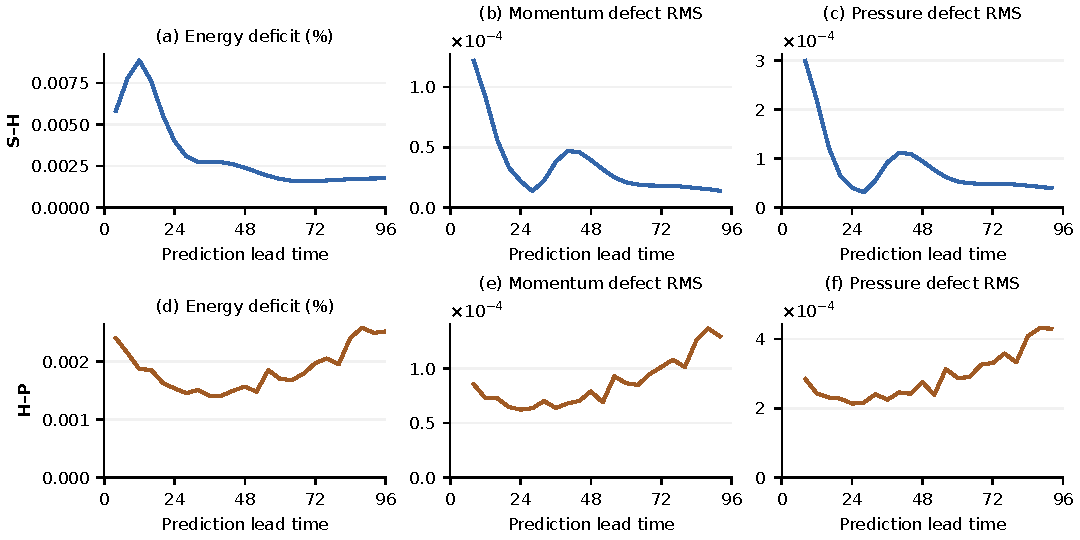
\includegraphics[width=\linewidth]{figures/fusion_defects_compact.pdf}
\caption{Additional effects of Square T2-C fusion with the 24-neighbor
initial stencil. Rows correspond to S--H (top) and H--P (bottom);
columns show normalized energy deficit $d_E$ in percent, momentum-defect
RMS, and pressure-defect RMS. Each curve averages all 16 windows at each
prediction lead time. Energy uses steps 1--24; residuals use steps 2--23.
Residual RMS is computed over the interior wake before window averaging.
The energy deficit is relative to weighted candidate energies, not
reference-energy error; residual defects are not total residuals.
Axes use panel-specific scales.}
\label{fig:fusion_energy_defects_supp}
\end{figure}

\FloatBarrier
% Replace the internal-routing portion of experimental_diagnostics.tex.
% The former fusion identities and Square diagnostics must be included
% only in the routing/fusion appendix, not repeated here.
% Existing labels are retained for compatibility. Requires amsmath,
% booktabs, and graphicx; reuses the two original routing PDFs.

\section{Internal expert routing: protocols and supplementary results}
\label{app:routing_physics}

\subsection{Circular: internal expert utilization}
\label{app:internal_routing}

This study characterizes correction-expert selection and weight allocation
inside individual regime-local specialists, rather than E2 selection
between specialists. We first define the sampling protocol and metrics,
then distinguish aggregate utilization, parameter-dependent allocation,
and variation along autonomous rollouts. The results describe the
evaluated checkpoints and windows, not all trained configurations.

\paragraph{Checkpoints and sampling protocol.}
We analyze frozen original Circular Hopf and Periodic specialists,
not the repaired three-seed models. Periodic is evaluated on 13 fixed
windows at each of four held-out Reynolds numbers, giving 52 windows
with $K=48$. Hopf uses five windows at each of three held-out Reynolds
numbers, giving 15 windows with $K=56$. These differ from the controlled
local reevaluation in Appendix~\ref{app:circular}.
We record one routing decision per output step at the first integration
stage, giving 2496 Periodic and 840 Hopf records per channel, rather
than counting every intermediate right-hand-side evaluation.
The statistics pool these records; overlapping windows are not treated
as independent trajectories. No routing diagnostic is used for
checkpoint selection.

\paragraph{Selection frequency and mixing weight.}
For each channel, let $I_{n,e}$ indicate whether routed expert $e$ is
selected at record $n$, including group identity in the expert index.
For $N$ records, define
\begin{equation}
f_e=\frac{1}{2N}\sum_{n=1}^{N}I_{n,e},
\qquad \sum_e f_e=1,
\label{eq:app_routing_frequency}
\end{equation}
where the factor two accounts for Top-2 activation at each record.
This is the fraction of selected expert slots, not the fraction of
time steps at which an expert is active. The mean routing mass is
\begin{equation}
m_e=\frac{1}{N}\sum_{n=1}^{N}\omega_{n,e}I_{n,e},
\label{eq:app_routing_mass}
\end{equation}
where $\omega_{n,e}$ is the final mixing coefficient, including the
scaling of the routed component. Unselected experts retain zero
frequency and mass. For these two checkpoints, the shared component
has coefficient $4/7$ and the routed Top-2 component has total
coefficient $3/7$, so $\sum_e m_e=3/7$.
The shared expert is excluded from the routed-expert counts below.
Routing mass quantifies weight allocation, not expert-output magnitude;
an expert's weight is not itself a measure of its physical contribution.
Identifiers such as \texttt{g0:e0} are local routed-expert labels and
do not denote the shared expert.

\paragraph{Selection diversity.}
With $N_E$ routed experts available to a channel, define
\begin{equation}
H=-\frac{\sum_{e:f_e>0}f_e\log f_e}{\log N_E},
\qquad 0\leq H\leq1.
\label{eq:app_routing_entropy}
\end{equation}
This entropy measures dispersion of activation frequencies, not mixing
weights or temporal switching. We also count distinct unordered Top-2
pairs, retaining group identity, and the fraction of records assigned
to the most frequent pair. An expert is counted as active if selected
at least once in the evaluated records.

\begin{table}[tbp]
\centering\small
\setlength{\tabcolsep}{5pt}
\caption{Post-hoc Circular internal-routing statistics. Active experts
are reported relative to all available routed experts; the shared
expert is excluded. Pair counts retain group identity. Dominant-pair
share is the fraction of records using the most frequent unordered
pair, and $H$ is activation-frequency entropy.}
\label{tab:internal_routing_summary}
\begin{tabular}{@{}llrrrr@{}}
\toprule
Specialist & Channel & \shortstack{Active\\experts}
& \shortstack{Distinct\\Top-2 pairs}
& \shortstack{Dominant-pair\\share (\%)} & $H$\\
\midrule
Hopf & Velocity & 2/6 & 1 & 100.00 & 0.387\\
& Pressure & 2/6 & 1 & 100.00 & 0.387\\
\addlinespace
Periodic & Velocity & 18/18 & 33 & 16.27 & 0.929\\
& Pressure & 14/18 & 16 & 31.25 & 0.784\\
\bottomrule
\end{tabular}
\end{table}

\paragraph{Periodic: broad but channel-dependent utilization.}
Table~\ref{tab:internal_routing_summary} shows that Periodic activates
all available velocity experts and most pressure experts. Velocity
selection is more dispersed than pressure selection, with more distinct
pairs, a smaller dominant-pair share, and higher utilization entropy.
Figure~\ref{fig:periodic_internal_routing} separates group frequencies
from routed-expert masses across the four held-out Reynolds numbers.
The group-selection frequencies vary across parameters, while the
channel-specific masses reveal how the routed weight is distributed.
These are utilization patterns, not assignments of physical mechanisms
to individual experts.

\paragraph{Hopf: fixed support with nonuniform weights.}
Hopf has a single group by architecture; the absence of group switching
is therefore not evidence that a learned multi-group router has collapsed.
Within that group, the observed velocity pair is $(e_1,e_3)$ and the
pressure pair is $(e_2,e_4)$ at every recorded step. Unlike the single-group
architecture, this fixed pair selection is an empirical observation on
the evaluated windows. A separate stage-wise check also found the same
pairs across all four Runge--Kutta stages.

Velocity expert $e_3$ receives approximately $99.93\%$ of the routed
mass, and pressure expert $e_2$ receives $84.16\%$. These percentages
are relative to the routed component, not the complete correction
including the shared expert. The secondary pressure expert $e_4$
has a mean mass that increases across the three evaluated Reynolds
numbers, so fixed support does not imply constant weight allocation.
For a fixed pair, both activation frequencies equal $1/2$ and
$H=\log 2/\log 6\simeq0.387$, regardless of how uneven their weights
are. Thus the entropy in the table does not indicate pair switching
or balanced expert contributions.

\paragraph{Allocation along Periodic rollouts.}
Figure~\ref{fig:periodic_routing_step} reports the mean routed-expert
mass at each normalized prediction position $k/48$, averaging the same
52 windows. It complements the parameter-wise statistics by showing
allocation along the autonomous rollout. Since the windows are not
aligned by physical oscillation phase, these profiles cannot establish
phase-specific expert specialization. Nor do aggregate utilization
statistics establish a causal accuracy benefit; that question requires
the controlled prediction comparisons rather than expert counts alone.

\begin{figure}[tbp]
\centering
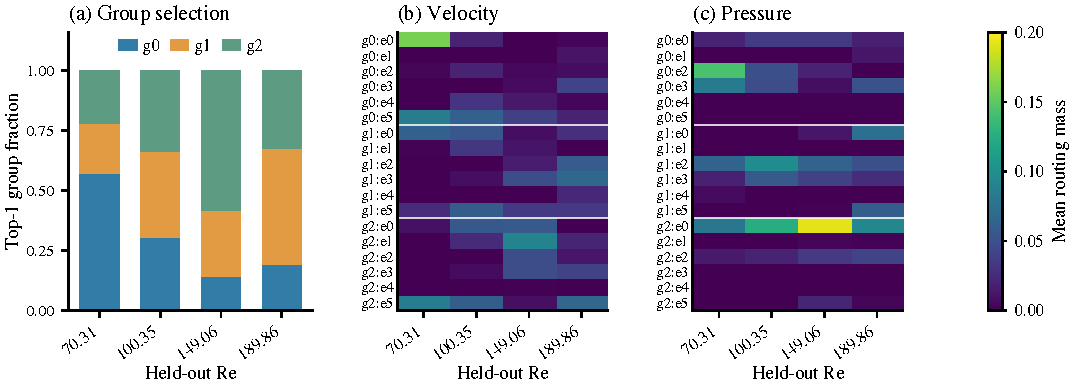
\includegraphics[width=\linewidth]{figures/periodic_internal_routing.pdf}
\caption{Parameter-dependent internal routing of the frozen Circular
Periodic specialist. (a) Top-1 group-selection frequencies.
(b,c) Mean routed-expert mass for velocity and pressure, respectively.
Records are collected at the first integration stage of each output
step over 13 windows per Reynolds number. Expert labels are local to
each group and channel; the shared component is not shown.}
\label{fig:periodic_internal_routing}
\end{figure}

\begin{figure}[tbp]
\centering
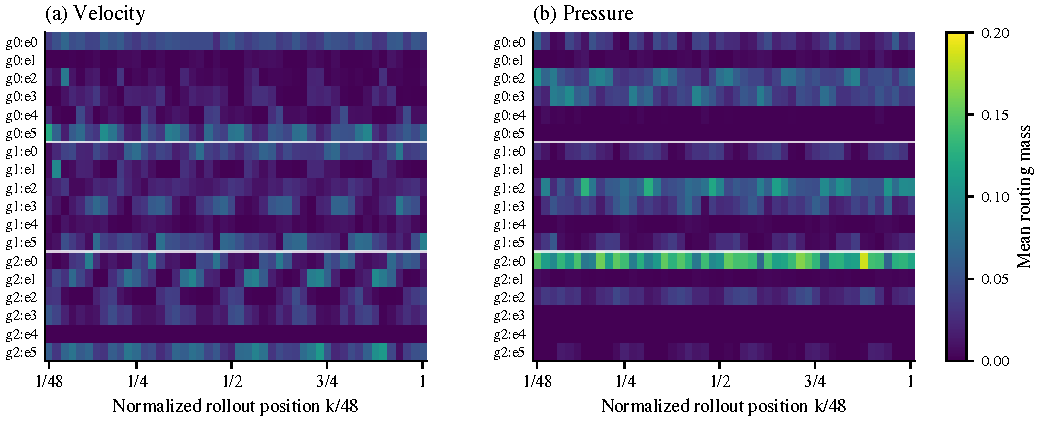
\includegraphics[width=\linewidth]{figures/periodic_rollout_step_routing.pdf}
\caption{Periodic routed-expert mass along autonomous rollouts.
Each column averages records at the same output step across 52 windows;
all routed experts are retained. The horizontal coordinate $k/48$
denotes normalized prediction position, not physical oscillation phase.
Masses include the routed-component scaling and exclude the shared
expert.}
\label{fig:periodic_routing_step}
\end{figure}

\FloatBarrier
% Replace appendix/experimental_cost.tex. Existing labels are retained.
\section{Computational cost and timing boundaries}
\label{app:parameter_counts}

We separate three questions: how many trainable parameters are used
per routing decision, how long the implemented local prediction paths
take, and how a warm specialist compares with a historical CFD run over
the same physical interval. Parameter accounting covers Circular H/P;
both timing studies cover Circular Periodic only. No Square or Pinball
runtime or complete hierarchical-pipeline speedup is inferred.

\subsection{Circular H/P: parameter utilization}

Total parameters count unique trainable parameters in each analyzed
specialist. Active parameters count unique trainable parameters used
by one batch-size-one prediction-path routing decision, not their union
across a batch, trajectory, or all Runge--Kutta stages. Included modules
are the encoder and refinement blocks, executed routers, the selected
group's shared experts, channel-specific Top-2 velocity and pressure
experts, and the learned pressure correction. Fixed POD bases, projected
operators, normalization statistics, and non-trainable buffers are excluded.

\begin{table}[tbp]
\centering
\caption{Circular trainable and per-decision active parameter counts.
Counts refer to unique trainable parameters, not FLOPs or memory usage.}
\label{tab:parameter_counts}
\begin{tabular}{@{}lrrr@{}}
\toprule
Specialist & Total trainable & Active prediction & Active fraction\\
\midrule
Hopf & 31,810,392 & 14,165,816 & 44.53\%\\
Periodic & 48,617,547 & 8,308,959 & 17.09\%\\
\bottomrule
\end{tabular}
\end{table}

Table~\ref{tab:parameter_counts} quantifies sparse use of the available
trainable capacity. It does not imply proportional reductions in storage,
operation count, or latency. The Dense control matches the active neural
parameter budget, not total model capacity or computational cost; it is
not identified with the older Vanilla-FNN-MoE, DataOnly-MoE, or Global MoE
configurations.

\subsection{Circular Periodic: local prediction latency}
\label{app:cost_local_latency}

\paragraph{Protocol and timing boundary.}
The native local-model comparison uses Circular Periodic seed 1248,
batch size one, $K=48$, three warm-up runs, and ten timed repetitions.
It includes modal rollout, feature generation, data transfers,
algebraic pressure reconstruction, all-step physical decoding, and
pressure gauge correction. It excludes physical-history encoding, E2
selection, descriptor construction, T2-C fusion, model/data loading,
and error computation. Thus it measures a local prediction path,
not a single neural forward pass or the complete hierarchy.

\begin{table}[tbp]
\centering\small
\caption{Native Circular Periodic local prediction cost at $K=48$.
Times are medians over ten repetitions after three warm-ups.
GPU memory denotes peak allocated bytes, not total device or host memory.}
\label{tab:local_latency}
\begin{tabular}{@{}lrrr@{}}
\toprule
Model & Median time (s) & GPU peak (bytes) & Time / Dense\\
\midrule
Proposed & 2.1848 & 204,238,336 & 3.32\\
Dense & 0.6579 & 43,111,936 & 1.00\\
Structured & 0.8652 & 43,316,736 & 1.32\\
\bottomrule
\end{tabular}
\end{table}

\paragraph{Interpretation.}
The proposed implementation is slower than both controls and has higher
peak allocated GPU memory in this measurement
(Table~\ref{tab:local_latency}). The native Galerkin NumPy path executes
on the CPU, but these aggregate timings do not isolate the contribution
of individual modules or establish the cause of the latency difference.
Sparse parameter activation therefore provides no measured runtime
advantage over Dense under this implementation and timing boundary.

\subsection{Circular Periodic: physical-input timing and historical FOM reference}
\label{app:cost_fom_reference}

\paragraph{Matched physical interval.}
A separate measurement of the original Periodic specialist (seed 1248)
adds full-size physical-history encoding and history right-hand-side
construction. At $\mathrm{Re}=70.314635$, the frozen first legal
$K=48$ window spans $t=1384.49597$ to $1983.19690$, a duration of
$598.70093$ physical time units. Its input consists of three
POD-reconstructed history frames on 97,368 points. All 48 predicted
velocity and pressure fields are decoded, with pressure gauge correction.
The model and input fields are resident before timing; acquiring the
history is not timed. This boundary differs from the local-model
comparison in Appendix~\ref{app:cost_local_latency}.

\paragraph{ROM measurement.}
On an RTX 4090 with a Xeon Platinum 8358P host, using one CPU numerical
thread, batch size one, three warm-ups, ten repetitions, and CUDA
synchronization, the median is $2.18747$ s. The mean is $2.18729$ s,
the sample standard deviation is $0.00462$ s, and the range is
$2.18034$--$2.19550$ s. Loading the model and inputs, writing predictions
to disk, E2 selection, descriptor construction, and T2-C fusion are
outside this measurement. Offline model construction and training are
also outside the online prediction timing.

\paragraph{Historical FOM measurement.}
The corresponding production OpenFOAM log contains 4,692 solver steps
and a ClockTime difference of 1,996 s. The largest discrepancy between
the ROM and FOM interval endpoints is $2.3\times10^{-5}$ physical time
units, attributable to stored timestamp precision. The production
solver used one process on a Core i5-14600K VMware host with 16 vCPUs
and at most five concurrent cases. This hardware information comes
from a subsequent source audit, not a contemporaneous controlled
benchmark. There is one FOM timing realization. The recorded interval
includes native solver field writes but excludes meshing, initialization,
periodic detection, and subsequent VTK/NPZ conversion.

\paragraph{Scope of the wall-time ratio.}
The ratio $1996/2.18747\simeq912.5$ compares a historical production
FOM interval with a warm, physical-input/physical-output local specialist.
It provides a case-specific online cost reference, not a controlled
end-to-end speedup: hardware, concurrency, repetition counts, and I/O
boundaries differ. In particular, the ROM measurement excludes outer
selection and fusion and cannot represent the cost of advancing and
assembling two specialists. A fully paired Top-2 end-to-end timing
under matched compute and I/O conditions remains unmeasured.


\end{document}
